\documentclass[12pt,a4paper,twoside,openright]{report} %deleting opentight solves black rectangle on the end of overfull lines
\let\openright=\cleardoublepage



%%% Choose a language %%%

\newif\ifEN
\ENtrue   % uncomment this for english
%\ENfalse   % uncomment this for czech

%%% Configuration of the title page %%%

\def\ThesisTitleStyle{mff} % MFF style
%\def\ThesisTitleStyle{cuni} % uncomment for old-style with cuni.cz logo
%\def\ThesisTitleStyle{natur} % uncomment for nature faculty logo

\def\UKFaculty{Faculty of Mathematics and Physics}
%\def\UKFaculty{Faculty of Science}

\def\UKName{Charles University in Prague} % this is not used in the "mff" style

% Thesis type names, as used in several places in the title
\def\ThesisTypeTitle{\ifEN BACHELOR THESIS \else BAKALÁŘSKÁ PRÁCE \fi}
%\def\ThesisTypeTitle{\ifEN MASTER THESIS \else DIPLOMOVÁ PRÁCE \fi}
%\def\ThesisTypeTitle{\ifEN RIGOROUS THESIS \else RIGORÓZNÍ PRÁCE \fi}
%\def\ThesisTypeTitle{\ifEN DOCTORAL THESIS \else DISERTAČNÍ PRÁCE \fi}
\def\ThesisGenitive{\ifEN bachelor \else bakalářské \fi}
%\def\ThesisGenitive{\ifEN master \else diplomové \fi}
%\def\ThesisGenitive{\ifEN rigorous \else rigorózní \fi}
%\def\ThesisGenitive{\ifEN doctoral \else disertační \fi}
\def\ThesisAccusative{\ifEN bachelor \else bakalářskou \fi}
%\def\ThesisAccusative{\ifEN master \else diplomovou \fi}
%\def\ThesisAccusative{\ifEN rigorous \else rigorózní \fi}
%\def\ThesisAccusative{\ifEN doctoral \else disertační \fi}



%%% Fill in your details %%%

% (Note: \xxx is a "ToDo label" which makes the unfilled visible. Remove it.)
\def\ThesisTitle{{Simulations of dynamics of ultra-cold quantum plasma}}
\def\ThesisAuthor{{Andrej Rendek}}
\def\YearSubmitted{{2022}}

% department assigned to the thesis
\def\Department{{Department of Surface and Plasma Science}}
% Is it a department (katedra), or an institute (ústav)?
\def\DeptType{{Department}}

\def\Supervisor{{Mgr. Michal Hejduk, Ph.D.}}
\def\SupervisorsDepartment{{Department of Surface and Plasma Science}}

% Study programme and specialization
\def\StudyProgramme{{Physics}}
\def\StudyBranch{{Physics}}

\def\Dedication{%
A would like to show my appreciation for\dots}

\def\AbstractEN{%
We investigate the confinement of charged particles in an oscillating electromagnetic field, intending to trap electrons and calcium ions simultaneously. The theoretical part of this thesis focuses on the derivation of exact and effective equations of motion in a single frequency quadrupole trap. We show a general treatment of stability in such a field. Passing attained knowledge onto two-frequency trapping, which is much more suitable for confining two species with widely different charge-to-mass ratios. We follow up by studying the stability of electrons, employing computer simulations in the ideal two-frequency Paul trap. Our ambition is to identify a stable configuration minimizing electrons' temperature. We create multiple ion Coulomb crystals and examine the effect of their presence on electrons' stability. These efforts support the development of an experiment with the ambition to create and study quantum plasma. The composition of this experiment is outlined here as well.
}

\def\AbstractCS{%
}

% 3 to 5 keywords (recommended), each enclosed in curly braces.
% Keywords are useful for indexing and searching for the theses by topic.
\def\Keywords{%
{Ion trapping,} {Coulomb crystal,} {Two frequency Paul trap}
}

% If your abstracts are long and do not fit in the infopage, you can make the
% fonts a bit smaller by this setting. (Also, you should try to compress your abstract more.)
% Alternatively, consider increasing the size of the page by uncommenting the
% geometry modification in thesis.tex.
\def\InfoPageFont{}
%\def\InfoPageFont{\small}  %uncomment to decrease font size

\ifEN\relax\else
% If you are writing a czech thesis, you additionally need to fill in the
% english translation of the metadata here!
\def\ThesisTitleEN{\xxx{Thesis title in English}}
\def\DepartmentEN{\xxx{Name of the department in English}}
\def\DeptTypeEN{\xxx{Department}}
\def\SupervisorsDepartmentEN{\xxx{Superdepartment}}
\def\StudyProgrammeEN{\xxx{study programme}}
\def\StudyBranchEN{\xxx{study branch}}
\def\KeywordsEN{%
\xxx{{key} {words}}
}
\fi


\usepackage{isomath}

\usepackage[a-2u]{pdfx}

\ifEN\else\usepackage[czech,shorthands=off]{babel}\fi
\usepackage[utf8]{inputenc}
\usepackage[T1]{fontenc}

% See https://en.wikipedia.org/wiki/Canons_of_page_construction before
% modifying the size of printable area. LaTeX defaults are great.
% If you feel it would help anything, you can enlarge the printable area a bit:
%\usepackage[textwidth=390pt,textheight=630pt]{geometry}
% The official recommendation expands the area quite a bit (looks pretty harsh):
%\usepackage[textwidth=145mm,textheight=247mm]{geometry}

%%% FONTS %%%
\usepackage{lmodern} % TeX "original" (this sets up the latin mono)
\usepackage[LGRgreek]{mathastext} % for nomal font in math mode

% Optionally choose an override for the main font for typesetting
\usepackage[mono=false]{libertinus} % popular for comp-sci (ACM uses this)
%\usepackage{tgschola} % Schoolbook-like (gives a bit of historic feel)
%\usepackage[scale=0.96]{tgpagella} % Palladio-like (popular in formal logic).

% Optionally choose a custom sans-serif fonts (e.g. for figures and tables).
% Default sans-serif font is usually Latin Modern Sans. Some font packages
% (e.g. libertinus) replace that with a better matching sans-serif font.
\usepackage{tgheros} % recommended and very readable (Helvetica-like)
%\usepackage{FiraSans} % looks great
% DO NOT typeset the main text in sans-serif font!
% The serifs make the text easily readable on the paper.

% IMPORTANT FONT NOTE: Some fonts require additional PDF/A conversion using
% the pdfa.sh script. These currently include only 'tgpagella'; but various
% other fonts from the texlive distribution need that too (mainly the Droid
% font family).


% some useful packages
\usepackage{microtype}
\usepackage{amsmath,amsfonts,amsthm,bm,physics}
\usepackage{graphicx}
\usepackage{xcolor}
\usepackage{booktabs}
\usepackage{caption}
\usepackage{subcaption}
\usepackage{floatrow}
\usepackage{float} %figures on exact spots
\usepackage{nicefrac, xfrac}
\usepackage{verbatim}
\usepackage{siunitx}
\usepackage{hyperref}
\usepackage{titlesec}
\usepackage{footmisc}


% load bibliography tools
\usepackage[backend=bibtex,natbib,style=numeric,sorting=none]{biblatex}
% alternative with alphanumeric citations (more informative than numbers):
%\usepackage[backend=bibtex,natbib,style=alphabetic]{biblatex}
%
% alternatives that conform to iso690
% (iso690 is not formally required on MFF, but may help elsewhere):
%\usepackage[backend=bibtex,natbib,style=iso-numeric,sorting=none]{biblatex}
%\usepackage[backend=bibtex,natbib,style=iso-alphabetic]{biblatex}
%
% additional option choices:
%  - add `giveninits=true` to typeset "E. A. Poe" instead of full Edgar Allan
%  - `terseinits=true` additionaly shortens it to nature-like "Poe EA"
%  - add `maxnames=10` to limit (or loosen) the maximum number of authors in
%    bibliography entry before shortening to `et al.` (useful when referring to
%    book collections that may have hundreds of authors)
%  - for additional flexibility (e.g. multiple reference sections, etc.),
%    remove `backend=bibtex` and compile with `biber` instead of `bibtex` (see
%    Makefile)
%  - `sorting=none` causes the bibliography list to be ordered by the order of
%    citation as they appear in the text, which is usually the desired behavior
%    with numeric citations. Additionally you can use a style like
%    `numeric-comp` that compresses the long lists of citations such as
%    [1,2,3,4,5,6,7,8] to simpler [1--8]. This is especially useful if you plan
%    to add tremendous amounts of citations, as usual in life sciences and
%    bioinformatics.
%  - if you don't like the "In:" appearing in the bibliography, use the
%    extended style (`ext-numeric` or `ext-alphabetic`), and add option
%    `articlein=false`.
%
% possibly reverse the names of the authors with the default styles:
%\DeclareNameAlias{default}{family-given}

% load the file with bibliography entries
\addbibresource{refs}

% remove this if you won't use fancy verbatim environments
\usepackage{fancyvrb}

% remove this if you won't typeset TikZ graphics
\usepackage{tikz}
\usetikzlibrary{positioning} %add libraries as needed (shapes, decorations, ...)

% remove this if you won't typeset any pseudocode
\usepackage{algpseudocode}
\usepackage{algorithm}

% remove this if you won't list any source code
\usepackage{listings}


\hypersetup{unicode}
\hypersetup{breaklinks=true}

\usepackage[noabbrev]{cleveref}


% remove this before submitting
\usepackage[textsize=tiny, backgroundcolor=yellow!25, linecolor=black!25]{todonotes}
\newcommand{\xxx}[1]{\textcolor{red!}{#1}}

 % remove this before compiling the final version


% use this for typesetting a chapter without a number, e.g. intro and outro
\def\chapwithtoc#1{
\chapter*{#1}
\addcontentsline{toc}{chapter}{#1}
}

% If there is a line/figure overflowing into page margin, this will make the
% problem evident by drawing a thick black line at the overflowing spot. You
% should not disable this.
\overfullrule=3mm

% The maximum stretching of a space. Increasing this makes the text a bit more
% sloppy, but may prevent the overflows by moving words to next line.
\emergencystretch=1em

\ifEN
\theoremstyle{plain}
\newtheorem{thm}{Theorem}
\newtheorem{lemma}[thm]{Lemma}
\newtheorem{claim}[thm]{Claim}
\newtheorem{defn}{Definition}
\theoremstyle{remark}
\newtheorem*{cor}{Corollary}
\else
\theoremstyle{plain}
\newtheorem{thm}{Věta}
\newtheorem{lemma}{Lemma}
\newtheorem{claim}{Tvrzení}
\newtheorem{defn}{Definice}
\theoremstyle{remark}
\newtheorem*{cor}{Důsledek}
\fi

\newenvironment{myproof}{
  \par\medskip\noindent
  \textit{\ifEN Proof \else Důkaz \fi}.
}{
\newline
\rightline{$\qedsymbol$}
}

% want a different minus sign
\newcommand{\minus}{\scalebox{1.0}[1.2]{$ \ - \ $}}

% real/natural numbers
\newcommand{\R}{\mathbb{R}}
\newcommand{\N}{\mathbb{N}}
\newcommand{\Z}{\mathbb{Z}}

% tensor
\newcommand{\tensorq}[1]{\ensuremath{\mathbb{#1}}}      % tensorial quantity
\newcommand{\tensorc}[1]{\ensuremath{\mathrm{#1}}}      % tensorial quantity components 

% asymptotic complexity
\newcommand{\asy}[1]{\mathcal{O}(#1)}

% listings and default lstlisting config (remove if unused)
\DeclareNewFloatType{listing}{}
\floatsetup[listing]{style=ruled}

\DeclareCaptionStyle{thesis}{style=base,font={small,sf},labelfont=bf,labelsep=quad}
\captionsetup{style=thesis}
\captionsetup[algorithm]{style=thesis,singlelinecheck=off}
\captionsetup[listing]{style=thesis,singlelinecheck=off}

% Uncomment for table captions on top. This is sometimes recommended by the
% style guide, and even required for some publication types.
%\floatsetup[table]{capposition=top}
%
% (Opinionated rant:) Captions on top are not "compatible" with the general
% guideline that the tables should be formatted to be quickly visually
% comprehensible and *beautiful* in general (like figures), and that the table
% "head" row (with column names) should alone communicate most of the content
% and interpretation of the table. If you just need to show a long boring list
% of numbers (because you have to), either put some effort into showing the
% data in an attractive figure-table, or move the data to an attachment and
% refer to it, so that the boredom does not impact the main text flow.
%
% You can make the top-captions look much less ugly by aligning the widths of
% the caption and the table, with setting `framefit=yes`, as shown below.  This
% additionally requires some extra markup in your {table} environments; see the
% comments in the example table in `ch2.tex` for details.
%\floatsetup[table]{capposition=top,framefit=yes}

\ifEN\floatname{listing}{Listing}
\else\floatname{listing}{Výpis kódu}\fi
\lstset{ % use this to define styling for any other language
  language=C++,
  tabsize=2,
  showstringspaces=false,
  basicstyle=\footnotesize\tt\color{black!75},
  identifierstyle=\bfseries\color{black},
  commentstyle=\color{green!50!black},
  stringstyle=\color{red!50!black},
  keywordstyle=\color{blue!75!black}}

% Czech versions of the used cleveref references (It's not as convenient as in
% English because of declension, cleveref is limited to sg/pl nominative. Use
% plain \ref to dodge that.)
\ifEN\relax\else
\crefname{chapter}{kapitola}{kapitoly}
\Crefname{chapter}{Kapitola}{Kapitoly}
\crefname{section}{sekce}{sekce}
\Crefname{section}{Sekce}{Sekce}
\crefname{subsection}{sekce}{sekce}
\Crefname{subsection}{Sekce}{Sekce}
\crefname{subsubsection}{sekce}{sekce}
\Crefname{subsubsection}{Sekce}{Sekce}
\crefname{figure}{obrázek}{obrázky}
\Crefname{figure}{Obrázek}{Obrázky}
\crefname{table}{tabulka}{tabulky}
\Crefname{table}{Tabulka}{Tabulky}
\crefname{listing}{výpis}{výpisy}
\Crefname{listing}{Výpis}{Výpisy}
\floatname{algorithm}{Algoritmus}
\crefname{algorithm}{algoritmus}{algoritmy}
\Crefname{algorithm}{Algoritmus}{Algoritmy}
\newcommand{\crefpairconjunction}{ a~}
\newcommand{\crefrangeconjunction}{ a~}
\fi

%one further subsection
\titleclass{\subsubsubsection}{straight}[\subsection]

\newcounter{subsubsubsection}[subsubsection]
\renewcommand\thesubsubsubsection{\thesubsubsection.\arabic{subsubsubsection}}
\renewcommand\theparagraph{\thesubsubsubsection.\arabic{paragraph}} % optional; useful if paragraphs are to be numbered

\titleformat{\subsubsubsection}
  {\normalfont\normalsize\bfseries}{\thesubsubsubsection}{1em}{}
\titlespacing*{\subsubsubsection}
{0pt}{3.25ex plus 1ex minus .2ex}{1.5ex plus .2ex}

\makeatletter
\renewcommand\paragraph{\@startsection{paragraph}{5}{\z@}%
  {3.25ex \@plus1ex \@minus.2ex}%
  {-1em}%
  {\normalfont\normalsize\bfseries}}
\renewcommand\subparagraph{\@startsection{subparagraph}{6}{\parindent}%
  {3.25ex \@plus1ex \@minus .2ex}%
  {-1em}%
  {\normalfont\normalsize\bfseries}}
\def\toclevel@subsubsubsection{4}
\def\toclevel@paragraph{5}
\def\toclevel@paragraph{6}
\def\l@subsubsubsection{\@dottedtocline{4}{7em}{4em}}
\def\l@paragraph{\@dottedtocline{5}{10em}{5em}}
\def\l@subparagraph{\@dottedtocline{6}{14em}{6em}}
\makeatother

\setcounter{secnumdepth}{4}
\setcounter{tocdepth}{4} % use this file for various custom definitions

\begin{document}

% the layout is mandatory, edit only in dire circumstances

\pagestyle{empty}
\hypersetup{pageanchor=false}
\begin{center}

% top part of the layout, this actually differs between faculties

\def\ThesisTitleXmff{%
  \ifEN
    \centerline{\mbox{
\includegraphics[width=166mm]{img/logo-en.pdf}}}
  \else
    \centerline{\mbox{
\includegraphics[width=166mm]{img/logo-cs.pdf}}}
  \fi
  \vspace{-8mm}\vfill%
  {\bf\Large\ThesisTypeTitle}
  \vfill%
  {\LARGE\ThesisAuthor}\par
  \vspace{15mm}%
  {\LARGE\bfseries\ThesisTitle}
  \vfill%
  \Department}
\def\ThesisTitleCuniLogo#1{%
  {\large\UKName\par\medskip\par\UKFaculty }
  \vfill%
  {\bf\Large\ThesisTypeTitle}
  \vfill%
  \includegraphics[width=70mm]{#1}
  \vfill%
  {\LARGE\ThesisAuthor}\par
  \vspace{15mm}%
  {\LARGE\bfseries\ThesisTitle}
  \vfill%
  \Department\par}
\def\ThesisTitleXcuni{\ThesisTitleCuniLogo{img/uklogo.pdf}}
\def\ThesisTitleXnatur{\ThesisTitleCuniLogo{img/naturlogo.pdf}}

% choose the correct page and print it
\csname ThesisTitleX\ThesisTitleStyle\endcsname
% latex corner: X is the new @

\vfill

{
\centerline{\vbox{\halign{\hbox to 0.45\hsize{\hfil #}&\hskip 0.5em\parbox[t]{0.45\hsize}{\raggedright #}\cr
\ifEN Supervisor of the \ThesisGenitive thesis:
\else Vedoucí \ThesisGenitive práce: \fi
& \Supervisor \cr
\noalign{\vspace{2mm}}
\ifEN Study programme: \else Studijní program: \fi
& \StudyProgramme \cr
\noalign{\vspace{2mm}}
\ifEN Study branch: \else Studijní obor: \fi
& \StudyBranch \cr
}}}}

\vfill

\ifEN Prague \else Praha \fi
\YearSubmitted

\end{center}

\newpage

% remember to sign this!
\openright
\hypersetup{pageanchor=true}
\pagestyle{plain}
\pagenumbering{roman}
\vglue 0pt plus 1fill

\ifEN
\noindent
I declare that I carried out this \ThesisAccusative thesis independently, and only with the cited
sources, literature and other professional sources. It has not been used to obtain another
or the same degree.
\else
\noindent
Prohlašuji, že jsem tuto \ThesisAccusative práci vypracoval(a) samostatně a výhradně
s~použitím citovaných pramenů, literatury a dalších odborných zdrojů.
Tato práce nebyla využita k získání jiného nebo stejného titulu.
\fi

\ifEN
\medskip\noindent
I understand that my work relates to the rights and obligations under the Act No.~121/2000 Sb.,
the Copyright Act, as amended, in particular the fact that the Charles
University has the right to conclude a license agreement on the use of this
work as a school work pursuant to Section 60 subsection 1 of the Copyright~Act.
\else
\medskip\noindent
Beru na~vědomí, že se na moji práci vztahují práva a povinnosti vyplývající
ze zákona č. 121/2000 Sb., autorského zákona v~platném znění, zejména skutečnost,
že Univerzita Karlova má právo na~uzavření licenční smlouvy o~užití této
práce jako školního díla podle §60 odst. 1 autorského zákona.
\fi

\vspace{10mm}


\ifEN
\hbox{\hbox to 0.5\hsize{%
In \hbox to 6em{\dotfill} date \hbox to 6em{\dotfill}
\hss}\hbox to 0.5\hsize{\dotfill\quad}}
\smallskip
\hbox{\hbox to 0.5\hsize{}\hbox to 0.5\hsize{\hfil Author's signature\hfil}}
\else
\hbox{\hbox to 0.5\hsize{%
V \hbox to 6em{\dotfill} dne \hbox to 6em{\dotfill}
\hss}\hbox to 0.5\hsize{\dotfill\quad}}
\smallskip
\hbox{\hbox to 0.5\hsize{}\hbox to 0.5\hsize{\hfil Podpis autora\hfil}}
\fi

\vspace{20mm}
\newpage

% dedication

\openright

\noindent
\Dedication

\newpage

% mandatory information page

\openright

\vbox to 0.49\vsize{\InfoPageFont
\setlength\parindent{0mm}
\setlength\parskip{5mm}

\ifEN Title: \else Název práce: \fi
\ThesisTitle

\ifEN Author: \else Autor: \fi
\ThesisAuthor

\DeptType:
\Department

\ifEN Supervisor: \else Vedoucí bakalářské práce: \fi
\Supervisor, \SupervisorsDepartment

\ifEN Abstract: \AbstractEN \else Abstrakt: \AbstractCS \fi

\ifEN Keywords: \else Klíčová slova: \fi
\Keywords

\vss}\ifEN\relax\else\nobreak\vbox to 0.49\vsize{\InfoPageFont
\setlength\parindent{0mm}
\setlength\parskip{5mm}

Title:
\ThesisTitleEN

Author:
\ThesisAuthor

\DeptTypeEN:
\DepartmentEN

Supervisor:
\Supervisor, \SupervisorsDepartmentEN

Abstract:
\AbstractEN

Keywords:
\KeywordsEN

\vss}
\fi

\newpage

\openright
\pagestyle{plain}
\pagenumbering{arabic}
\setcounter{page}{1}


\tableofcontents

\chapwithtoc{Introduction}

The practical aim of this thesis is to contribute to the development of an experiment initiated by my supervisor Mgr. Michal Hejduk, Ph.D. In this experiment, we wish to create and study the properties of a quite unusual type of plasma, Coulomb crystal. Coulomb crystals are mostly stationary structures of ions characterized by large coupling parameter $\Gamma$, representing the ratio between electrostatic and kinetic energy of ions. These structures have been extensively studied now for decades. Our ambition is to introduce electrons to such a crystal, which to my knowledge, hasn't been achieved yet. We will be aiming for sub-kelvin temperatures when electrons de Broglie wavelength would be bigger than the distance between them, forming so-called Fermi gas. Creating a Coulomb crystal means confining a certain number of charged particles in bounded space. The first thing standing in our way is the Earnshaw theorem, stating that there is no stable electrostatic configuration of charged particles. Of course, we are not about to give up just yet. Therefore we must try our luck outside the realm of electrostatics. Here we have already been presented with two well-established ways of storing charged particles. One utilizes an axial magnetic field to confine particles in a radial direction, and a rapidly changing electric field for confinement in an axial direction. This approach developed by H.G. Dehmelt is called the Penning trap. The second option to restrict the movement of charged particles in all directions is to use the dynamic electric field solely. Such a trap bears the name of Wolfgang Paul, hence the Paul trap. Both these gentlemen were, for their efforts in this field, awarded a shared Nobel prize for physics in 1989. The ions in our experiment will be laser-cooled, which would be disturbed by a magnetic field due to Zeeman splitting. Ergo we are left with the latter method. My job will be to make a computer simulation of an ion crystal with electrons inside a Paul trap trying to optimize the parameters of the trap to attain the lowest possible temperature of electrons, hopefully reaching the point of crystalization for such a system.
\chapter{Theoretical introduction}
\label{chap:intro}

In this chapter, we introduce concepts essential for understanding this thesis's concerns. This chapter is divided into several subsections. \footnote{\xxx{In the first subsection, we are going to discuss the basic principles of plasma physics. In the following subsection, we will talk about the motion of a charged particle inside the Paul trap. Next, we will introduce the idea of laser cooling. And finally, in the last subsection, we will present our approach to simulating such a system, entering this thesis's practical component.}} \todo{the sections in the first two chapters will probably be rearranged}

\section{Coulomb crystal}
Most of the ordinary matter has a crystal or rather polycrystal structure. Meaning its elementary constituents (atoms, molecules, ions) create an ordered formation repeating itself, in the case of crystals up to macroscopic scales. The shape of these structures \cite{drewsen2003ion} is essentially dictated by the wave function overlap. A CC orders itself differently. An average distance between ions in a CC is usually \cite{thompson2015ion} five orders of magnitude larger than it is for atoms in solid matter. On this scale are quantum effects negligible, and ions are merely pushed away from each other by classical Coulomb interaction. Therefore they need an external force to keep them together, which is provided by a trapping potential in our case. However, these structures can also be found in nature, namely in the cores of white dwarfs and crusts of neutron stars.

\subsection{Plasma}
The broadest definition of plasma is to identify it as ionized gas \cite{fitzpatrick2014plasma}\xxx{\dots}. The standard definition is more strict by demanding quasineutrality and collective behavior as well. We will call such plasma as \emph{conventional plasma}\todo{check the usage of this term}. Quasineutrality suggests the same ion and electron concentrations over the whole volume. By this merit, a CC is far from being a conventional plasma as it is composed exclusively of positive ions.\todo{what is collective behavior, coupling parameter, maybe other plasma parameters, strongly coupled plasma, maybe Rydberg ions}

\section{Ion trapping}
Here we introduce the concept of trapping a single ion by a quickly oscillating field. We will tightly follow a classic textbook \cite{gerlich1992inhomogeneous} in the whole section, starting by writing the equation of motion.

\subsection{Equation of motion}
Let us consider a particle with mass $M$, charge $Q$, and position denoted by vector $\vb{r}$. We insert such a particle into the external time-dependent electromagnetic field described by $\vb{E}(t,\vb{r})$ and $\vb{B}(t,\vb{r})$. The Lorentz force gives the equation of motion:
\begin{equation}
	M \vb{\ddot{r}} = Q \left[\vb{E}(t,\vb{r}) + \vb{\dot{r}} \times \vb{B}(t,\vb{r})\right].
\end{equation}
Since we are not using any external magnetic field, and while trapping a particle in a compact space, we usually deal with small velocities. Therefore we neglect\footnote{This and other approximations are further discussed in the section \ref{sec:simulation}.} the effect of the term $\vb{\dot{r}} \times \vb{B}$, which means that the equation of motion simplifies to:
\begin{equation}
	M \vb{\ddot{r}} = Q \ \vb{E}(t,\vb{r}).
\end{equation}
We further assume that the electric field is composed of static and time-dependent parts. We are looking for a simple periodic time-dependency. A typical way to model such behavior would be $\vb{E}(t) \sim \cos(\Omega_1 t)$, giving us:
\begin{equation}
	\vb{E}(t,\vb{r}) = \vb{E_s}(\vb{r}) + \vb{E_0}(\vb{r}) \cos(\Omega_1 t),
\end{equation}
and following equation of motion:
\begin{equation}
	\label{equation of motion}
	M \vb{\ddot{r}} = Q \left[ \vb{E_s}(\vb{r}) + \vb{E_0}(\vb{r}) \cos(\Omega_1 t) \right].
\end{equation}

\subsection{Effective potential}
Dealing with such rapidly changing non-autonomous differential equations can be a riot, although it is possible to solve them analytically for special boundary conditions, as will be discussed further. By a lucky chance, we are not always interested in exact solutions while trapping ions. The relevance often lies in the time-averaged effect of a swiftly changing field. With that in mind, we will now try to derive \emph{effective potential} fulfilling precisely this role.

Let's consider initial conditions: $\vb{r}(0) = \vb{r_0}$ and $\vb{\dot{r}}(0) = 0$. For the case of an oscillating electric field with homogeneous amplitude $\vb{E_0}(\vb{r}) = const$, we obtain a trivial solution:
\begin{equation}
	\label{solution for homogenious field}
	\vb{r}(t) = \vb{r_0} \minus \vb{A} \cos(\Omega_1 t),
\end{equation}
where the vector: 
\begin{equation}
	\label{oscillation amplitude}
	\vb{A} \equiv \vb{A}(\vb{r}) = \frac{Q \vb{E_0}(\vb{r})}{m \Omega_1^2},
\end{equation}
is an amplitude of oscillation around the initial position of the particle. The crucial consequence of this result is that we can further restrict the motion of a particle by increasing the frequency of field oscillation. Of course, the situation changes when we bring a small inhomogeneity into the field. Here comes our first leap of fate by assuming that our defining relation for the amplitude of oscillation \eqref{oscillation amplitude} won't be affected by such inhomogeneity. Instead, the particle will drift slowly towards the weaker field region, minimizing its mean potential energy. Motivated by these two assumptions, we can try to find a solution to the equation of motion in the form:
\begin{equation}
	\label{motion separation}
	\vb{r}(t) = \vb{R_0}(t) + \vb{R_1}(t),
\end{equation}
where $\vb{R_0}(t)$ represents consequence of smooth drift and $\vb{R_1}(t)$ stands for rapid oscillation, expressed as:
\begin{equation}
	\label{oscillation motion}
	\vb{R_1}(t) = \minus \vb{A} \cos(\Omega_1 t).
\end{equation}
If the field amplitude $\vb{E_0}(\vb{r})$ varies smoothly with regards to the space dimension, we can get by just with its first-order Taylor expansion around $\vb{R_0}$:
\begin{equation}
	\label{field expansion}
	\vb{E_0}(\vb{R_0}(t) \minus \vb{A} \cos(\Omega_1 t)) \approx \vb{E_0}(\vb{R_0}(t)) \minus(\vb{A} \cdot \nabla) \vb{E_0}(\vb{R_0}(t)) \cos(\Omega_1 t) + \dots.
\end{equation}
Substituting \eqref{motion separation} and \eqref{field expansion} into equation of motion \eqref{equation of motion} \textit{(omitting currently uninteresting static term $\vb{E_s}$)}, we get:
\begin{multline}
	M \big( \vb{\ddot{R}_0(t)} + \vb{\ddot{R}_1(t)} \big) = Q \cos(\Omega_1 t) \big[ \vb{E_0(\vb{R_0}(t))} \\ \minus (\vb{A} \cdot \nabla) \vb{E_0(\vb{R_0}(t))} \cos(\Omega_1 t)  \big].
\end{multline}
Presuming slow spacial variation of vectorfield $\vb{E_0}(\vb{r})$ implies: \\ $|\vb{\ddot{A}}| \ll |\vb{\dot{A}}| \Omega_1 \ll |\vb{A}| \Omega_1^2$, which we can exploit in time derivative of quickly oscillating term $\vb{R_1}(t)$ \eqref{oscillation motion}, giving us:
\begin{equation}
	\vb{\ddot{R}_1} = \minus \vb{\ddot{A}} \cos(\Omega_1 t) + 2 \Omega_1 \vb{\dot{A}} \sin(\Omega_1 t) + \vb{A} \Omega_1^2 \cos(\Omega_1 t) \approx \vb{A} \Omega_1^2 \cos(\Omega_1 t)
\end{equation}
Further substituting for amplitude of oscillation $\vb{A}$ from \eqref{oscillation amplitude} continuing in the spirit of time-averaging:
\begin{equation}
	\vb{A} = \frac{q \vb{E_0}(\vb{r})}{M \Omega_1^2} \approx \frac{q \vb{E_0}(\vb{R_0}(t))}{M \Omega_1^2},
\end{equation}
which transfers into $\vb{R_1}$ as:
\begin{equation}
	\label{oscillation motion approx}
	\vb{R_1}(t) = \minus \frac{Q \vb{E_0}(\vb{R_0}(t))}{M \Omega_1^2} \cos(\Omega_1 t). 
\end{equation}
Terms in the equation of motion with dependence on $cos(\Omega_1 t)$ cancel each other out and by using a vector identity:
\begin{equation}
	\label{vector identity}
	(\vb{E_0} \cdot \nabla) \vb{E_0} = \frac{1}{2} \nabla E_0^2 \minus \vb{E_0} \times (\nabla \times \vb{E_0}) = \frac{1}{2} \nabla E_0^2,
\end{equation}
where the second equality follows from Maxwell equation for quasistatic field: \\ $\nabla \times \vb{E_0} = 0$. By replacing term $\cos^2(\Omega_1 t)$ with its mean value $\langle\cos^2(\Omega_1 t)\rangle = \nicefrac{1}{2}$ we finally obtain:
\begin{equation}
	M \vb{\ddot{R}_0} = \frac{Q^2}{4 M \Omega_1^2} \nabla E_0^2.
\end{equation}
Now by resurrecting the static field term as $\vb{E_s} = \minus \nabla \Phi_s$, we can define the effective potential:
\begin{equation}
	\label{effective potential}
	V^*(\vb{R_0}) = \frac{Q^2 E_0^2(\vb{R_0})}{4 M \Omega_1^2} + q \Phi_s, 
\end{equation}
describing the time-averaged force on a charged particle:
\begin{equation}
	\label{effective equation of motion}
	M \vb{\ddot{R}_0} = \minus \nabla V^*(\vb{R_0}). 
\end{equation}
This equation is much easier to solve and discuss than the original equation of motion \eqref{equation of motion} as it does not involve any explicit time-dependency. After solving it, we can quickly obtain the term $\vb{R_1}(t)$ from \eqref{oscillation motion approx} and get an approximative solution to the original equation of motion. From the Fourier analyses of numerically exact solutions \cite{gerlich1992inhomogeneous} we know about the presence of higher-order terms: $$\vb{r}(t) = \vb{R_0}(t) + \vb{R_1}(t) + \vb{R_2}(t) + \dots,$$ where $\vb{R_2}(t) + \dots$ are referred to as micro oscillations. We must be careful about keeping the space variation of $\vb{E_0}(\vb{r})$ sufficiently small. Otherwise, these micro oscillations can become large enough to disturb the trajectory of a particle significantly.

\subsection{Adiabacity}
Let us examine the motion of a charged particle in derived effective potential. The first integral of the equation \eqref{effective equation of motion} is:
\begin{equation}
	\label{first integral of motion}
	\dfrac{1}{2}M R_0^2 + \dfrac{Q^2 E_0^2}{4 M \Omega_1^2} + Q\Phi_s = E_m,
\end{equation}
where $E_m = const$ is the total energy of a charged particle inside the trap. Furthermore, if we consider the average kinetic energy of the rapidly oscillatory motion:
\begin{equation}
	\left\langle \dfrac{1}{2} M R_1^2 \right\rangle = \dfrac{1}{2}M \dfrac{Q^2 E_0^2}{M^2 \Omega^4}\Omega^2 \langle sin^2(\Omega t) \rangle = \dfrac{Q^2 E_0^2}{4 M \Omega_1^2},
\end{equation}
we see that equation \eqref{first integral of motion} implies:
\begin{equation}
	\label{adiabatic constant}
	\dfrac{1}{2}M R_0^2 + \left\langle \dfrac{1}{2} M R_1^2 \right\rangle + Q\Phi_s = E_m,
\end{equation}
which means that if the necessary assumptions in the derivation of the effective potential are met, then the total time-averaged energy of the system is an adiabatic constant. This raises the question of whether there is a way to quantify a range of validity for the effective potential. There are more ways to approach this problem, but we will follow the one demonstrated in \cite{gerlich1992inhomogeneous}, kicking off the necessary condition for keeping just the first two terms in Taylor expansion \eqref{field expansion} of the field $\vb{E}(\vb{r})$. This condition is met if the change of the field is much smaller than the field itself over the scope of one rapid oscillation, meaning:
\begin{equation}
	|2(\vb{A} \cdot \nabla)\vb{E_0}| < |\vb{E_0}|.
\end{equation}
Inspired by this condition we define a new parameter $\eta$:
\begin{equation}
	\eta = \dfrac{|2(\vb{A} \cdot \nabla)\vb{E_0}|}{|\vb{E_0}|} = \dfrac{2Q|\nabla E_0|}{M\Omega_1^2},
\end{equation}
where the last equality follows after implementing \eqref{oscillation amplitude} and \eqref{vector identity}. We can use this parameter to check the extent of the effective pseudopotential, but it can be a good indicator of stable trapping conditions, as we will see further.

\subsection{Trap geometry}
Previously derived equations indirectly feature the potential $\Phi = \Phi_{rf} + \Phi_s$ as the dynamic and static electric intensities are $\vb{E_0}\cos(\Omega_1 t) = \minus\nabla \Phi_{rf}$ and $\vb{E_s} = \minus\nabla \Phi_s$. So to give these general equations some concrete shape, we need to find this potential. In our quasistationary treatment of the electric field, it means solving the Laplace equation for a given boundary condition. Writing a general solution to the Laplace equation is possible only for certain symmetries. One such is cylindrical symmetry, for which we can work out the solution by hand using a Fourier method of separating variables in polar coordinates $(x=r \cos\varphi, \ y=r \sin\varphi)$ as:
\begin{multline}
	\label{cylindrical symmetry potential}
	\Phi(r, \varphi) = C_0 + D_0 \ln(r) + \sum_{n \in \N} \big( \left[A_n r^{n} + B_n r^{-n} \right] \\ 
	\left[ C_n \sin(n\varphi) + D_n \cos(n\varphi) \right] \big),
\end{multline}
where $C_0$, $D_0$, $A_n$, $B_n$, $C_n$ and $D_n$ are coefficients that need to be determined from boundary conditions. 

\subsubsection{Multipole trap}
A multipole is one of Paul trap's classical, well-studied geometries. N-th order multipole consists of 2n linear electrodes arranged with a discrete cylindrical symmetry.
\begin{figure}[H]
\begin{subfigure}{.4\textwidth}
	\centering
	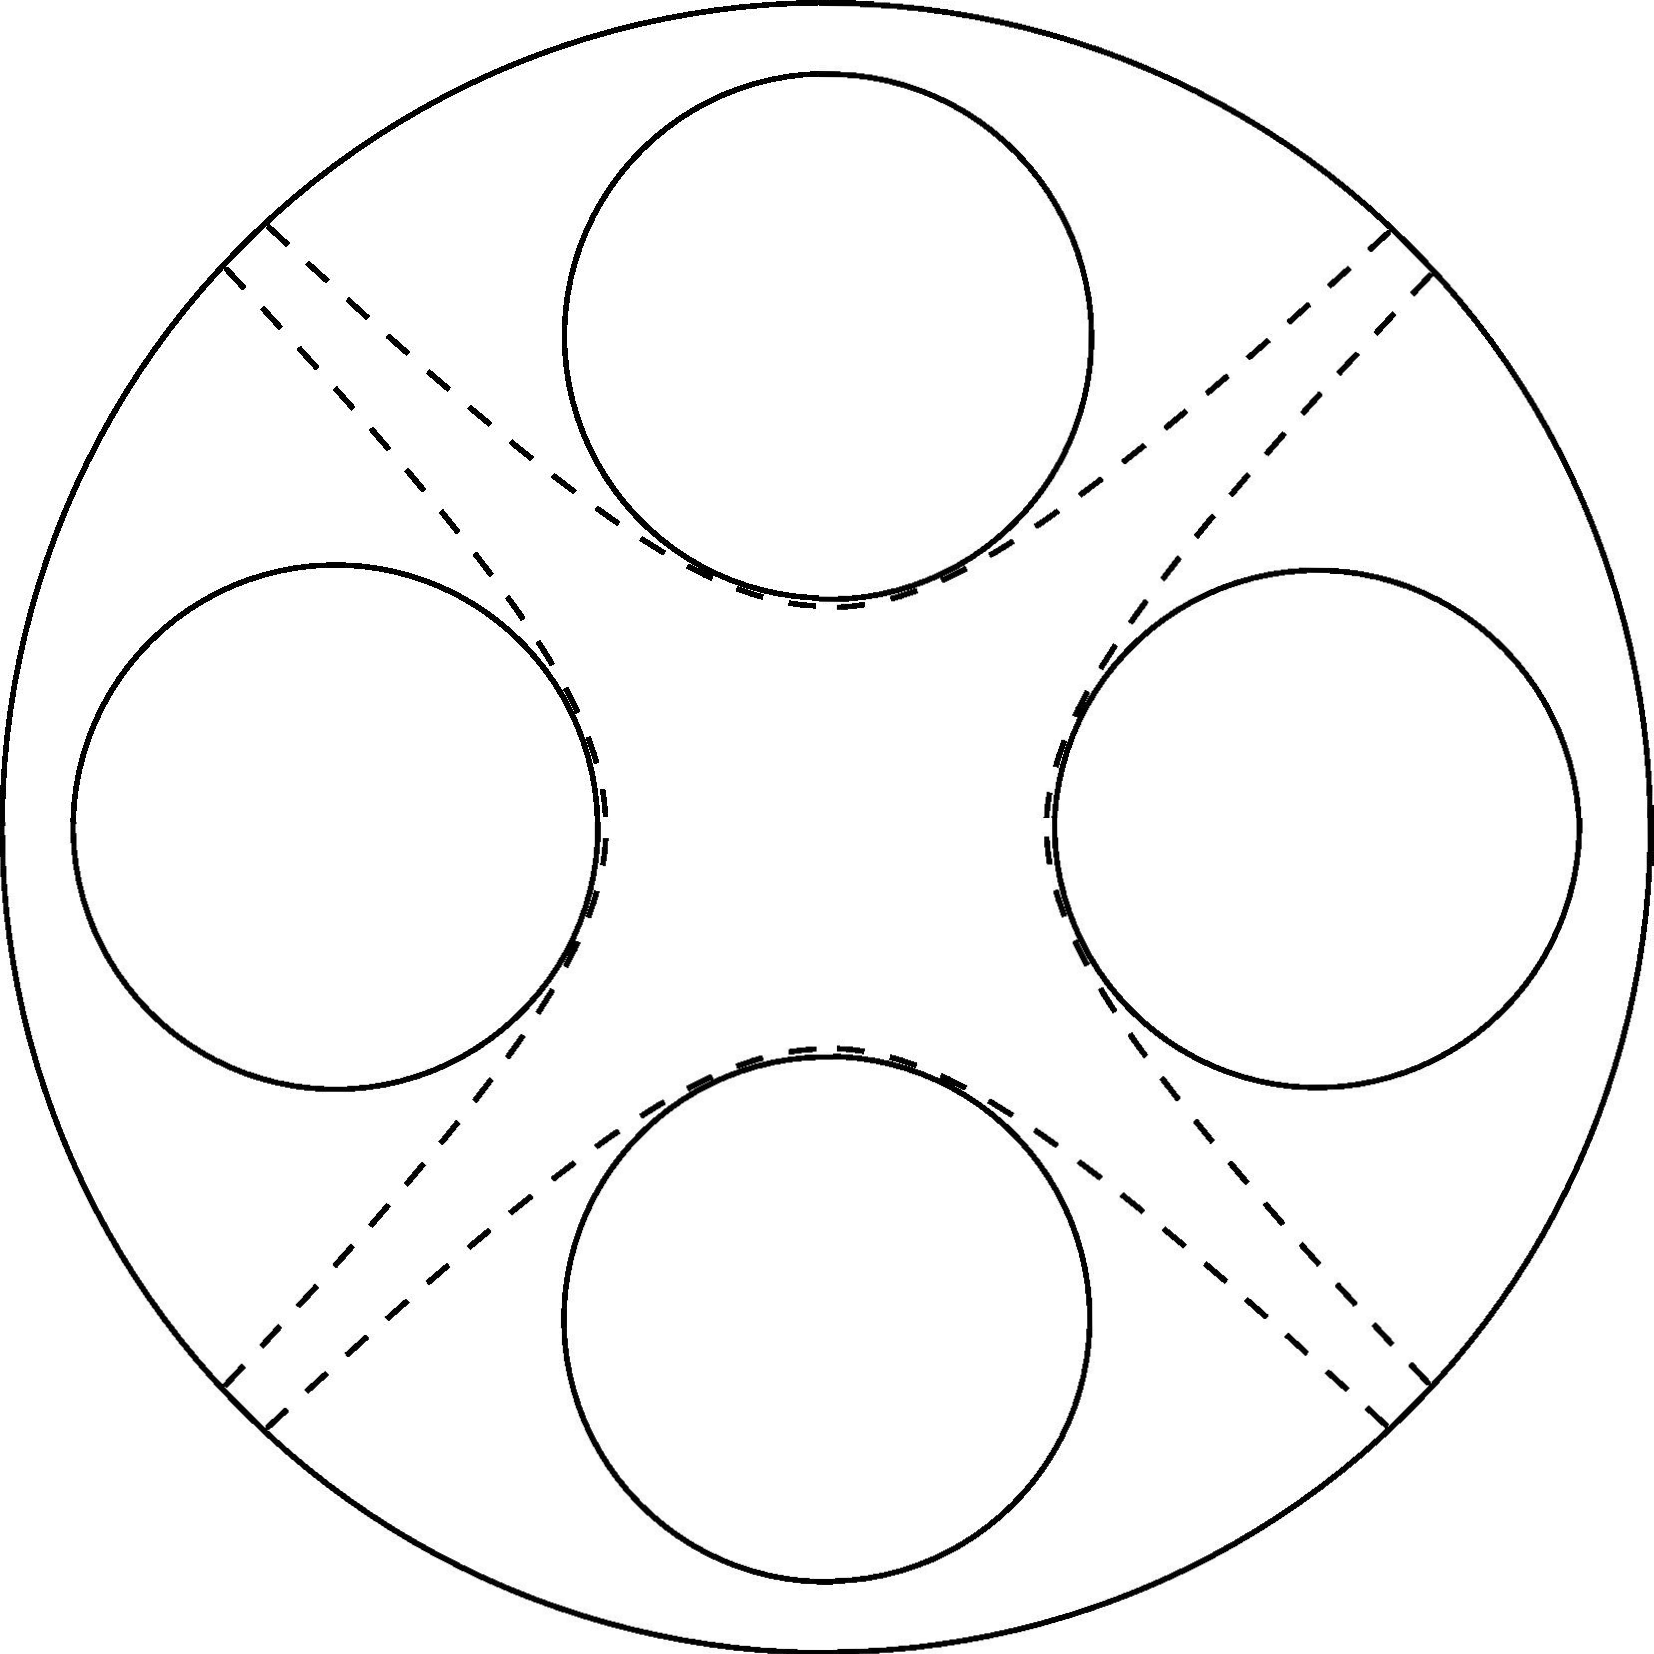
\includegraphics[width=\linewidth]{img/quadrupole_scheme.png}
	\caption{The scheme of quadrupole's cross-section. Adapted from \cite{FANGHANEL2017124}.}
	\label{fig:quadrupole scheme}
\end{subfigure}\hfill%
\begin{subfigure}{.47\textwidth}
	\centering
	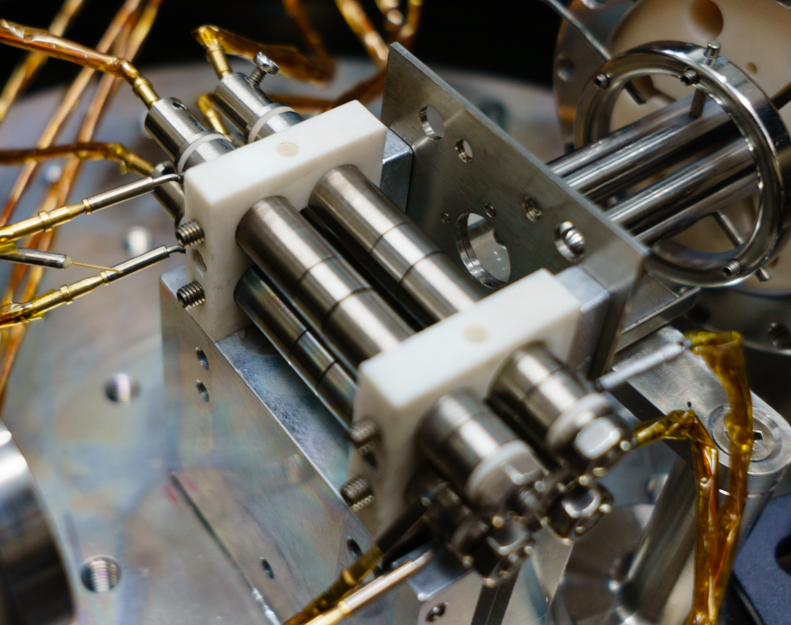
\includegraphics[width=\linewidth]{img/quadrupole.png}
	\caption{A photograph of linear quadrupole trap.}
	\label{fig:quadrupole picture}
\end{subfigure}
\caption{The quadrupole trap}
\label{fig:quadrupole}
\end{figure}
\todo{Do I need to cite somebody for \ref{fig:quadrupole picture}?}In the figure \ref{fig:quadrupole scheme}, we can see a comparison of a quadrupole trap's hyperbolical \textit{(dashed)} and linear \textit{(four circles)} electrode geometries. The quadrupole is already a very important geometry worth a special alias $\rightarrow$ the Paul trap, as will be pointed out shortly. We define a characteristic length of the multipole $\ell_0$, indicating the closest distance from the trap's center to an electrode. It is possible to obtain a potential of a multipole with infinitely long linear electrodes by applying boundary conditions \eqref{boundary condition n-pole} to a solution of Laplace equation with cylindrical symmetry \eqref{cylindrical symmetry potential}.
\begin{subequations}
\label{boundary condition n-pole}
\begin{align}
	\Phi(r,\varphi)\vert_{r=0}&=0, \\
	\Phi(r,\varphi)\vert_{r=\ell_0}&=\Phi_0 \cos(n\varphi),
\end{align}
\end{subequations}
where $\Phi_0 = V_0 + V_1 \cos(\Omega_1 t)$ is a potential applied on electrodes. Most of the coefficients in \eqref{cylindrical symmetry potential} get wiped out, and we end up with the potential of n-th order multipole $(n > 0)$ as:
\begin{equation}
	\label{potential n-pole}
	\Phi(r,\varphi) = \Phi_0 \hat{r}^n \cos(n\varphi),	
\end{equation}
where $\hat{r} = \nicefrac{r}{\ell_0}$. We get an electric intensity in polar coordinates as: 
\begin{equation}
	\vb{E}(r,\varphi) = \minus\nabla_{r\varphi} \Phi(r,\varphi),
\end{equation}
where $\nabla_{r\varphi} = \left[\dfrac{\partial}{\partial r}, \dfrac{1}{r} \dfrac{\partial}{\partial \varphi}\right]^\top$. We get:
\begin{equation}
\label{need this for norm(E_0)}
\vb{E}(r,\varphi) = \dfrac{\Phi_0}{\ell_0} n \hat{r}^{n-1} 
\begin{bmatrix}
	\minus\cos(n\varphi) \\
	\sin(n\varphi)
\end{bmatrix},
\end{equation}
which in the Cartesian representation takes the form \cite{gerlich1992inhomogeneous}:
\begin{equation}
\begin{bmatrix}
	E_x \\
	E_y
\end{bmatrix}
 = \dfrac{\Phi_0}{\ell_0} n \hat{r}^{n-1} 
\begin{bmatrix}
	\minus\cos\big((n \minus 1)\varphi\big) \\
	\sin\big((n \minus 1)\varphi\big)
\end{bmatrix}.
\end{equation}
After substituting for $\Phi_0$ we get equation of motion in variable $\vb{\hat{r}} = [\nicefrac{x}{\ell_0},\nicefrac{y}{\ell_0}]^\top$:
\begin{equation}
	\label{eq of motion multipole}
	\dfrac{d^2\vb{\hat{r}}}{dt^2} + F(t) \hat{r}^{n-1}
	\begin{bmatrix}
		\minus\cos\big((n \minus 1)\varphi\big) \\
		\sin\big((n \minus 1)\varphi\big)
	\end{bmatrix} = \vb{0},
\end{equation}
where we, for abbreviation, introduced the function:
\begin{equation}
	F(t) = n\dfrac{Q V_0}{M \ell_0^2} + n\dfrac{Q V_1}{M \ell_0^2} \cos(\Omega_1 t).
\end{equation}
We see that for $n = 2$ the equation of motion \eqref{eq of motion multipole} is linear. The same is clearly not true for the case of $n > 2$. That is why the motion in a quadrupole trap is easiest to describe, and we chose this geometry to study simultaneous electron-ion trapping in this thesis.

\subsubsubsection{Ideal quadrupole trap}
\label{sec:quadrupole trap}
We have already derived a equation of motion for single charged particle in a quadrupole trap $\rightarrow$ $n=2$ in \eqref{eq of motion multipole}. This equation gets further simplified by replacing linear electrodes with hyperbolical ones. With this change, the electric field gets scaled \cite{leefer2017investigation} by a factor $\nicefrac{1}{2}$, but foremost it loses the spatial dependence on the angle $\varphi$. In that case, the motion in the x and y directions stays decoupled, and we obtain an equation of motion in a variable $\vb{r} = (x,y)^\top$ for an idealized quadrupole trap:
\begin{equation}
	\label{eq of motion hyperbolic electrodes}
	M\vb{\ddot{r}} = \minus\dfrac{Q}{\ell_0^2} \big[V_0 + V_1 \cos(\Omega_1 t)\big] \vb{r}.
\end{equation}
The same equation describes motion in the z-direction, but with a rescaled right-hand side by the factor of $\minus 2$. We will take a closer look at the equation \eqref{eq of motion hyperbolic electrodes} in the section \ref{sec:mathieu equation}. While we are at it, we can take a step back and define the potential for the idealized quadrupole trap. Equation of motion in terms of such potential would be: $M\vb{\ddot{r}}(t) = \minus Q\nabla V(t,\vb{r})$, comparing with the \eqref{eq of motion hyperbolic electrodes} gives us desired potential:
\begin{equation}
	\label{ideal quadrupole potential}
	V(t,\vb{r}) = \left[V_0 + V_1 \cos(\Omega_1 t)\right] \dfrac{x^2+y^2 \minus 2z^2}{2\ell_0^2}
\end{equation}
Another essential subject we are interested in is the effective potential for this geometry. For that, we need to evaluate for $E_0$ in the equation \eqref{effective potential}. The value of $\vb{E_0}$ can be easily derived from \eqref{need this for norm(E_0)}, where for our case $\Phi_0 = \nicefrac{V_1}{2}$, as:
\begin{equation}
	\label{norm(E_0)}
	E_0 = \dfrac{V_1}{\ell_0^2} r,
\end{equation}
which means that the effective potential is:
\begin{equation}
	\label{effective potential hyperbolic}
	V^*(\vb{r}) = \dfrac{Q^2 V_1^2}{4\ell_0^4 M \Omega_1^2} r^2 + q\Phi_s.
\end{equation}

\subsubsection{Real geometry of our trap}
Since we want to implement laser cooling in our experiment, the Paul trap is not a viable option, as its apparatus would stand in the way of laser beams. For this reason, we will use surface electrodes where the particles levitate above the trap so that the ions will be accessible to us.
\begin{figure}[H]
\begin{subfigure}{.5\textwidth}
  \centering
  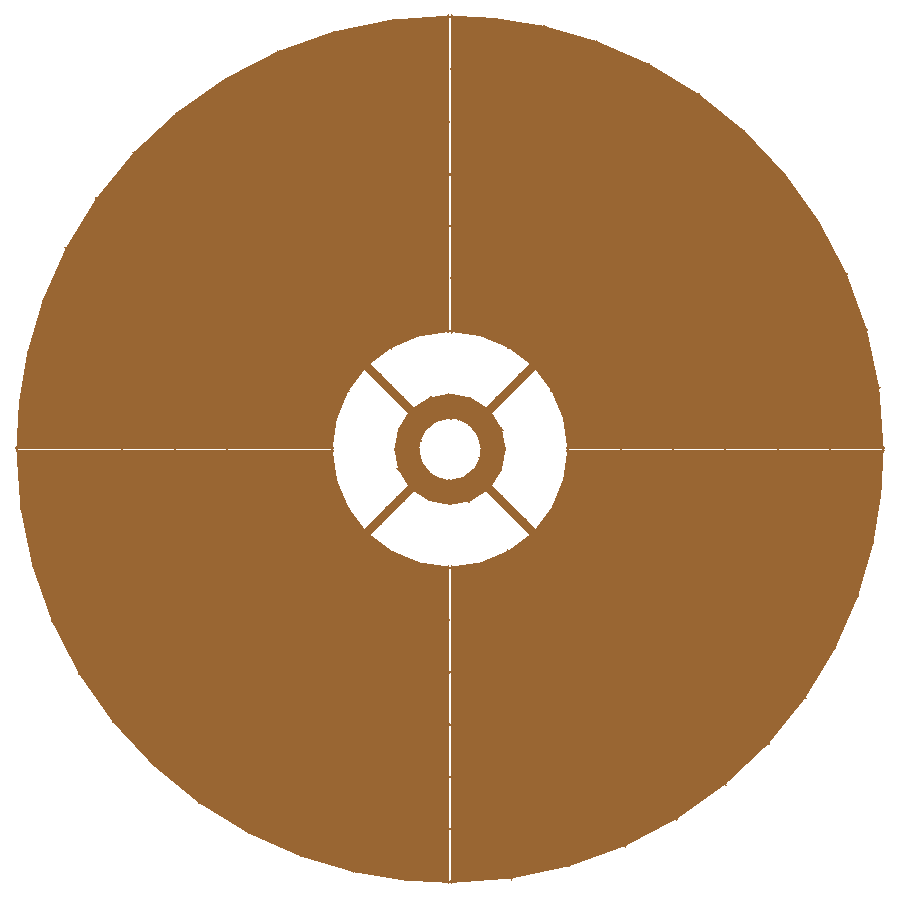
\includegraphics[width=\linewidth]{img/real_trap_geometry_1.pdf}
  \caption{Scheme of our planar trap}
  \label{fig:Real trap geometry 1}
\end{subfigure}%
\begin{subfigure}{.5\textwidth}
  \centering
  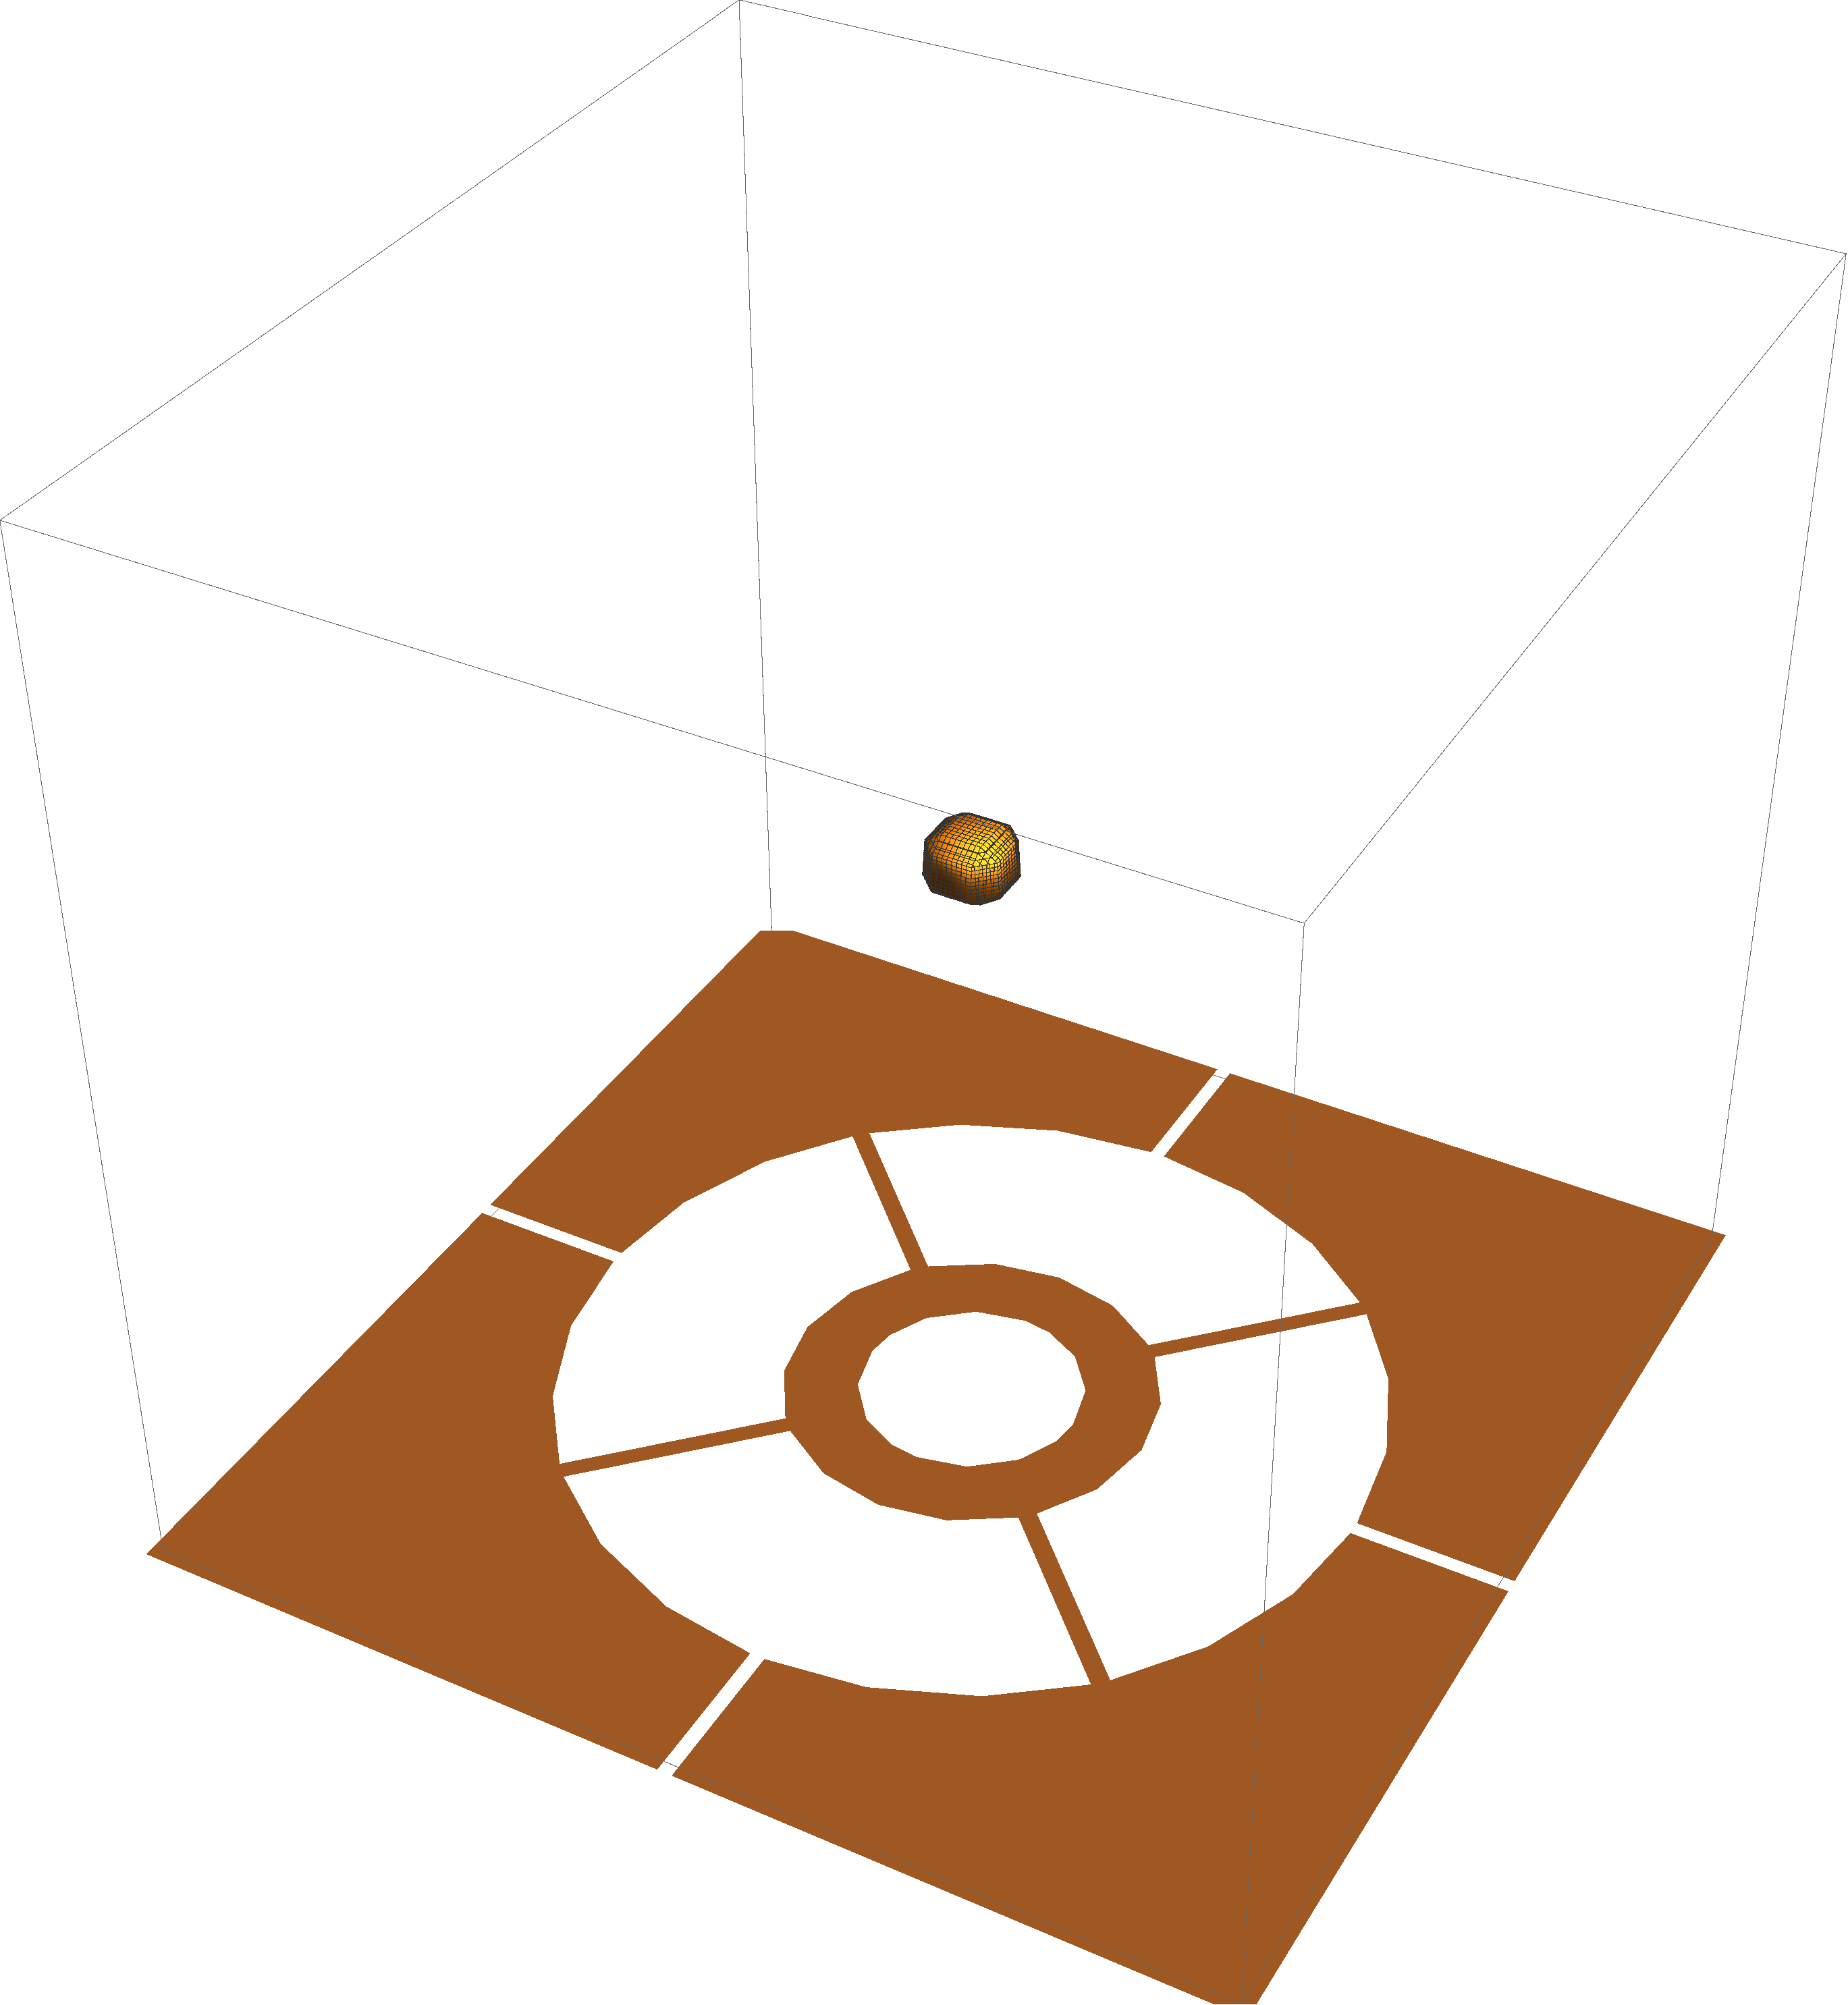
\includegraphics[width=\linewidth]{img/real_trap_geometry_2.pdf}  
  \caption{(3 x 3) millimeter segment of our trap with the potential well above it}
  \label{fig:Real trap geometry 2}
\end{subfigure}
\caption{Planar trap geometry}
\label{fig:planar trap geometry}
\end{figure}
Nevertheless, we will conduct our research in this thesis by examining the situation with the geometry of the ideal quadrupole trap with hyperbolic electrodes.

\subsection{Spring constant}
\label{sec:spring constant}
If we focus on the dynamic component of an effective potential \eqref{effective potential hyperbolic}, we can see that it is formally equivalent to a potential of a harmonic oscillator\footnote{Meaning a potential in the form: $V(\xi) = \dfrac{\kappa}{2} \xi^2$}. This encourages us to define a spring constant: 
\begin{equation}
	\label{spring constant}
	\kappa \equiv \dfrac{Q^2 V_1^2}{2\ell_0^4 M \Omega_1^2},
\end{equation}
characterizing the strength of trapping potential. The spring constant is closely related to a frequency of oscillation in a harmonic potential. Such frequency is called secular, denoted: 
\begin{equation}
	\label{secular frequency}
	\omega \approx \sqrt{\nicefrac{\kappa}{M}} = \nicefrac{Q V_1}{\sqrt{2}\ell_0^2 M \Omega_1}.
\end{equation}
The good news is that the spring constant does not depend on the charge sign, making it possible to trap electrons as well as ions. The bad news is that the spring constant depends on the charge-to-mass ratio $\nicefrac{Q}{M}$, making it practically very difficult to trap electrons and ions simultaneously. For our case of trapping Ca+ ions together with electrons, we get $\nicefrac{\kappa_{electron}}{\kappa_{ion}} = \nicefrac{M_{ion}}{M_{electron}} \approx 73000$ while we would like to achieve $\nicefrac{\kappa_{electron}}{\kappa_{ion}} \sim 10$ so that electron trajectories would ideally stay inside the ion crystal but at the similar scales. It seems that we have hit upon a huge snag with our approach. Fortunately, this does not mean we have to abandon the idea of RF trapping itself. Instead, we can improve on it by adding a second frequency, giving us the freedom to treat the stability of both species individually and making it possible to manage the desired ratio of spring constants. Two frequency Paul trap will be further discussed in section \ref{sec:two frequency trap}.

\xxx{We aim to create a Coulomb crystal and trap electrons within so that a cooled electron would spread its de Broglie's wavelength across multiple ions. For this, we need tighter confinement of electrons, but the ions must be close to each other as well. }

\subsection{Mathieu equation}
\label{sec:mathieu equation}
Let us reexamine our original equation of motion \eqref{equation of motion} for the case of a quadrupole trap with ideal hyperbolical electrodes. After time transformation $\tau = \nicefrac{\Omega_1 t}{2}$, the equation \eqref{eq of motion hyperbolic electrodes} molds into:
\begin{equation}
	\label{mathieu equation}
	\ddot{\vb{r}}(\tau) = \left[a \minus 2 q_1 \cos(2 \tau)\right] \vb{r},
\end{equation}
where:
\begin{subequations}
\begin{align}
	a &= \dfrac{4 Q V_0}{M \ell_0^2 \Omega_1^2}, \\
	q_1 &= \minus\dfrac{2 Q V_1}{M \ell_0^2 \Omega_1^2}.
\end{align}
\end{subequations}
The equation \eqref{mathieu equation} bears a name after E.L. Mathieu, who was the first to extensively study it in the context of vibrating membranes. It has an analytical solution \cite{5416839} in terms of special functions called Mathieu functions, denoted $ce_n$ and $se_n$, sometimes referred to as cosine-elliptic and sine-elliptic. The secular is given by \cite{gerlich1992inhomogeneous} the Dehmelt approximation:
\begin{equation}
	\omega \approx \frac{\Omega_1}{2} \sqrt{a + \frac{q_1^2}{2}}.
\end{equation}
If we apply no static field $a = 0$ the secular frequency is:
\begin{equation}
	\omega \approx \frac{\Omega_1}{2} \sqrt{\dfrac{q_1^2}{2}} = \dfrac{Q V_1}{\sqrt{2}\ell_0^2 M \Omega_1},
\end{equation}
which is in accordance with the result we attained with the spring constant of the harmonic pseudopotential.

\subsection{Stability} 
The stability of a linear system such as \eqref{mathieu equation} can be examined with the help of a robust theory for linear ordinary differential equations(ODEs) with periodic coefficients, which we do in section \ref{sec:floquet theory}. Nevertheless, we eventually want to study the trapping of multiple charged particles, and their mutual interaction razes the linearity of our equations. There is no single outright mathematical way to define the stability of a non-linear, non-autonomous system. Mathematical approaches might demand the boundedness of the solution in the phase space. Then we would talk about Lagrange stability \cite{bhatia2002stability}. Another approach would be to seek stable points and study what happens to the solutions starting in their proximity. This approach is referred to as Lyapunov stability \cite{lyapunov1992general}. We will use a simple but practical criterion for identifying stable solutions. A stable particle cannot vacate the internal dimension of the trap, meaning:
\begin{equation}
	\max\limits_{x \in \mathcal{L}}(r) \leq r_m < \ell_0,
\end{equation}
where $\mathcal{L}$ is the whole trajectory of the particle and $r_m$ is maximal allowed distance from the center of a trap. The drawback of this definition is that we must keep the simulation going long enough to account for the slowly diverging particles, and we are yet to determine the value of $r_m$. However, we can also characterize the mode for stable confinement in a more general manner \cite{gerlich1992inhomogeneous}. First, we limit ourselves to work within the condition for adiabaticity to ensure that the dynamic field does not continually augment the particle's energy. Then we can exploit the equation \eqref{adiabatic constant} in the following way. A stable particle must have no secular momentum $\vb{\dot{R}_0} = \vb{0}$ at the point $r_m$ to avoid collision with the electrode. The effective potential near the electrode must be greater than the adiabatic constant $E_m$. Otherwise, the potential will not be powerful enough to prevent rapid oscillatory motion from ejecting the particle out of the trap. Giving us the applicable inequality for stable confinement:
\begin{equation}
	\label{stability condition inequality}
	\dfrac{Q^2 E_0^2(r_m)}{4 M \Omega^2} + Q\Phi_s > E_m.
\end{equation}
We still need to find the right value for $r_m$. It has been established \cite{gerlich1992inhomogeneous} that $r_m = 0.8 \ \ell_0$ accomplishes adiabaticity for most cases, which we will also use as a stability condition in our simulations:
\begin{equation}
	\label{stability condition in simulation}
	\max\limits_{x \in \mathcal{L}}(r) \leq 0.8 \ \ell_0.
\end{equation}

\section{Laser cooling}
The Ca+ ion has an energy gap between the ground $(s_{\nicefrac{1}{2}})$ and one of its excited $(p_{\nicefrac{1}{2}})$ states with the value corresponding to the wavelength of $\SI{397}{\nano\meter}$ \cite{urabe1993laser}. By tuning the wavelength of our laser slightly below this transition energy, we can exploit the Doppler effect so that only ions moving towards the laser can experience radiation with the right frequency to excite them. After a brief time, the atom will deexcite, emitting a photon in a random direction. The only way the ion would still have the same momentum as before the absorption is if the photon was emitted exactly in the same direction as it was absorbed (as if the photon did not interact with the atom at all). But since the photon emission is isotropic, the ion will effectively slow down. This type of laser cooling is also known as \emph{Doppler cooling}. Detailed explanation can be found in \cite{alma990008711500106986}.   

\section{Desing of our experiment}

\chapter{Co-trapping of two different species}
\label{chap:co-trapping}

\section{Two frequency quadrupole Paul trap}
\label{sec:two frequency trap}
As was mentioned in the section \ref{sec:spring constant},
we can use two frequencies, each targeting to optimize the trapping of one species. Higher frequency $\Omega_2$ for trapping electrons, with the potential $V_2$ applied to the electrode. A lower frequency $\Omega_1$ with potential $V_1$ for trapping ions. We have already derived the ideal quadrupole potential for a single frequency case. Repeating the same process with the exception of using applied potential on the electrodes in the form $\Phi_0 = V_0 + V_1 \cos(\Omega_1 t) + V_2 \cos(\Omega_2 t)$, would yield two-frequency potential for an ideal quadrupole:
\begin{equation}
	\label{ideal quadrupole potential two frequency}
	V(t,\vb{r}) = \left[V_0 + V_1 \cos(\Omega_1 t) + V_2 \cos(\Omega_2 t)\right] \dfrac{x^2+y^2 \minus 2z^2}{2\ell_0^2}.
\end{equation}
We proceed in setting up a two-frequency trap as described in \cite{FOOT2018117, trypogeorgos2016cotrapping}. First, we must acknowledge that while higher frequency will have no significant impact on heavier ions, a light electron will experience the slower field to the full extent. Therefore we have to ensure that the trapping of electrons due to the higher frequency field is strong enough to withstand misguiding by the field with a lower frequency. We refer to this latent instability as the \emph{parametric excitation}. We can secure that to some extent by feeding potentials on electrodes in such a way that $V_1 \ll V_2$. We can provide potentials up to $V_2 \sim \SI{100}{\volt}$, and $V_1 \sim \SI{5}{\volt}$, in the conditions of our experiment. Let us now look at each frequency setup independently. Using \eqref{spring constant}, we get a ratio of spring constants:
\begin{equation}
	\label{two frequency ratio}
	\Kappa = \dfrac{\kappa_{el}(\Omega_2)}{\kappa_{ion}(\Omega_1)} \approx \dfrac{M_{ion}}{M_{el}} \left(\dfrac{V_2}{V_1}\dfrac{\Omega_1}{\Omega_2}\right)^2.
\end{equation}
The correct way to create a stable configuration of a two-frequency trap is to begin by finding the optimal parameters for the confinement of lighter species. Optimal trapping in a single frequency trap corresponds to \cite{gerlich1992inhomogeneous} $q_2 \approx 0.4$. Using \eqref{q_2}, with the choice of $V_2 = \SI{100}{\volt}$, we obtain optimal frequency for electron trapping as $\Omega_2 = \SI{1.88e10}{rad.s^{-1}}$. Now, we must choose the $\Omega_1$ and $V_1$ for ion trapping in a way that suppresses parametric heating of electrons. It is crucial to keep the electron's secular frequency higher than the driving frequency for ion confinement. Otherwise, the $\Omega_2$ frequency field would be too slow to save an electron from parametric excitation. So another condition that must be satisfied in two frequency trapping is:
\begin{equation}
	\label{frequency inequality}
	\Omega_1 \ll \omega_2 = \dfrac{Q V_2}{\sqrt{2} M_{el} \ell_0^2 \Omega_2},
\end{equation}
where the second equality follows from \eqref{secular frequency}. Unfortunately \cite{FOOT2018117}, we will not be able to forestall parametric heating all the time. In the case of $$\mu \Omega_1 = 2 \omega_2,$$
where $\mu \in \N$, occurs resonance of driving $\Omega_1$ and secular $\omega_2$ frequency, resulting in heating of lighter species. If substitute for $\omega_2$ from \eqref{secular frequency}, we get a set of unstable parameters $q_2$ characterized by the equation:
\begin{equation}
	\label{unstable q_2}
	q_2 = \sqrt{2}\mu\nicefrac{\Omega_1}{\Omega_2},
\end{equation}
which explains the origin of unstable tongues in stability diagrams; see \ref{chap:results} the last chapter.

We aim to create a Coulomb crystal and trap electrons within so that a cooled electron could spread its de Broglie wavelength across multiple ions. For this, we need tighter confinement of electrons, but the ions must also be close to each other. Lower frequency $\Omega_1$ means weaker ion confinement. Since we have not accounted for ion repulsion yet, we chose the frequency $\Omega_1$ corresponding to the spring ratio $\Kappa \approx 42$.

In the case of a quadrupole with perfectly hyperbolical electrodes we have a electric potential in the form:
\begin{equation}
	V(t, \vb{r}) = \bigg[ V_0 + V_1 cos(\Omega_1 t) + V_2 \cos(\Omega_2 t) \bigg] \frac{x^2 + y^2 \minus 2 z^2 }{2 \ell_0^2},
\end{equation}
where $V_0$ is an amplitude of static potential, $V_1$ of slower potential and $V_2$ is an amplitude of rapidly oscillating potential on the electrode. The equations of motion for a particle in such potential, after change of variable: $\tau = \nicefrac{t\Omega_2}{2}$ are:
\begin{subequations}
\label{eq of motion for simulation}
\begin{align}
	\ddot{x}(\tau) & = x(\tau) \bigg[ a \minus 2 q_1 \cos\left(2 \tau \nicefrac{\Omega_1}{\Omega_2} \right) \minus 2 q_2 \cos(2\tau) \bigg], \\
	\ddot{y}(\tau) & = y(\tau) \bigg[ a \minus 2 q_1 \cos\left(2 \tau \nicefrac{\Omega_1}{\Omega_2} \right) \minus 2 q_2 \cos(2\tau) \bigg], \\
	\label{studied eq of motion}
	\ddot{z}(\tau) & = \minus 2z(\tau) \bigg[ a \minus 2 q_1 \cos\left(2 \tau \nicefrac{\Omega_1}{\Omega_2} \right) \minus 2 q_2 \cos(2\tau) \bigg],
\end{align}
\end{subequations}
where $a$, $q_1$ and $q_2$ are dimensionless parameters:
\begin{subequations}
\label{Mathieu params}
\begin{align}
	\label{a}
	a & = 4 \dfrac{Q V_0}{M\Omega_2^2 \ell_0^2}, \\
	\label{q_1}
	q_1 & = \minus 2 \dfrac{Q V_1}{M\Omega_2^2 \ell_0^2}, \\
	\label{q_2}
	q_2 & = \minus 2 \dfrac{Q V_2}{M\Omega_2^2 \ell_0^2}.
\end{align}
\end{subequations}
Although we are not using any static potential, implying this, we keep it in our equations for generality.

Instead of solving exact equations of motion, we can simulate a charged particle in an effective potential, significantly reducing computational time. We will use this option while creating a Coulomb crystal. When trapping electrons, the condition \eqref{frequency inequality} must be satisfied hence we can use already derived single frequency effective potential \eqref{effective potential hyperbolic}:

\begin{equation}
	\label{electron pseudopotential}
	V_{el}^*(\vb{r}) = \frac{M_{el} \Omega_2^2 q_2^2}{16}(x^2 + y^2 + 4 z^2),
\end{equation}
where we have set the static field to zero and substituted for $q_2$ from \eqref{q_2}. Both frequencies will figure only in pseudopotential for ions. Let us remark that Mathieu parameters \eqref{Mathieu params} differ for the case of electron and ion by a factor of $\nicefrac{M_{el}}{M_{ion}}$. Using the Mathieu parameters evaluated for electrons, the pseudopotential for ions \cite{leefer2017investigation} is:

\begin{equation}
	\label{ion pseudopotential}
	V_{ion}^*(\vb{r}) = \frac{M_{el}^2 \Omega_2^2}{16 M_{ion}} \left( \left(\frac{\Omega_2}{\Omega_1}\right)^2 q_1^2 + q_2^2 \right) \left(x^2 + y^2 + 4z^2\right).
\end{equation}
 

\section{Floquet theory}
\label{sec:floquet theory}
Since the particle experiences the weakest confinement in the z-direction, we will examine this equation's properties. Floquet theory is a theory covering linear first-order ODEs with periodic coefficients. These are equations of the form:
\begin{equation}
	\label{Floquet structure}
	\dot{\vb{u}}(\tau) = \tensorq{F}(\tau) \vb{u}(\tau),
\end{equation}
where $\tensorq{F}$ is a matrix valued function with minimal period $T$. Let's illustrate this theory for the case of our differential equation. We begin by rewriting the equation \eqref{eq of motion for simulation} as one general system of two first-order differential equations written in the matrix form:
\begin{align}
\label{matrix mathieu}
	\frac{d}{d \tau}
	\begin{bmatrix}
		\zeta(\tau) \\
		\dot{\zeta}(\tau)
	\end{bmatrix}	
	&=
	\begin{bmatrix}
		0 & 1 \\
		\tilde{a} \minus 2 \tilde{q}_1 \cos\left(2 \tau \nicefrac{\Omega_1}{\Omega_2} \right) \minus 2 \tilde{q}_2 \cos(2\tau) & 0	
	\end{bmatrix}
	\begin{bmatrix}
		\zeta(\tau) \\
		\dot{\zeta}(\tau)
	\end{bmatrix},
\end{align}
where:
\begin{align}
	\label{xi variable}
	\zeta &\in \{x,y,z\}, \\
	\label{tilde params} 
	\{ \tilde{a}, \tilde{q}_1, \tilde{q}_2 \} &= \begin{cases}
		\{a, q_1, q_2\} &if \ (\zeta = x) \lor (\zeta = y), \\
		\minus 2 \{a, q_1, q_2\} &if \ (\zeta = z). 
	\end{cases}
\end{align}
This system \eqref{matrix mathieu} already has a structure of \eqref{Floquet structure}. Without the necessity of finding a solution to this system, we can acquire knowledge about its stability. The information we are interested in is whether a solution is bounded for a given set of parameters or not. In this section, we will limit ourselves to the driving frequencies, which can be represented as: $\nicefrac{\Omega_2}{\Omega_1} \equiv \nicefrac{m}{n}$, where $m$ and $n$ are integers and $\nicefrac{m}{n}$ is an irreducible fraction. Then the matrix in equation \eqref{matrix mathieu} is $T = m \pi$ periodic. As in \cite{leefer2017investigation}, we identify the edge of stability regions as a set of parameters for which a solution of \eqref{studied eq of motion} is a $2T$ periodic function\footnote{Note that such stability condition differs from the one we demand while simulating the motion of a particle. The periodic solution of equation of motion implies boundedness, but the value of this boundary might lie outside the physical dimensions of the trap. That is why we ought not to be surprised when we find some differences in stability diagrams, even for the simplest case of a single particle in the trap. \label{foot:different stability condition}} to our problem \eqref{matrix mathieu}. This allows us to seek a solution to our problem in the form:
\begin{equation}
	\label{Floquet ansatz}
	\zeta(\tau) = \sum_{k=-\infty}^{\infty} c_k \exp(i\frac{k}{m}\tau),
\end{equation}
where $c_k$ are constant coefficients. Substituting this into equation \eqref{matrix mathieu} yields an identity:

\begin{multline}
	\sum_{k=\minus\infty}^{\infty}\left[ \left(\tilde{a} \minus \dfrac{k^2}{m^2} \right)c_k \minus \tilde{q}_1 \left(c_{k-2n} + c_{k+2n} \right) \minus \tilde{q}_2 \left(c_{k-2m} + c_{k+2m} \right)  \right] \\ \exp(i\frac{k}{m}\tau) = 0,
\end{multline}
which holds for every $\tau$ only if each element of the sum is equal to zero. This relation can be written as:

\begin{equation}
	\label{Floquet edge eq}
	\tensorq{F} \cdot \begin{bmatrix}
	\vdots \\
	c_{k-1} \\
	c_{k} \\
	c_{k+1} \\
	\vdots
	\end{bmatrix} = \vb{0},
\end{equation}
where $\tensorq{F}$ is an infinite matrix with elements:

\begin{equation}
	\tensorq{F}_{i j} = \left[ \left(\tilde{a} \minus \dfrac{k^2}{m^2} \right)\delta_{i j} \minus \tilde{q}_1 \left(\delta_{i j-2n} + \delta_{i j+2n} \right) \minus \tilde{q}_2 \left(\delta_{i j-2m} + \delta_{i j+2m} \right)  \right],
\end{equation} 
where:
\begin{equation}
	\delta_{ij} = 
	\begin{cases}
		1 & i=j, \\
		0 & i \neq j.
	\end{cases}	
\end{equation}
The equation \eqref{Floquet edge eq} is equivalent to:
\begin{equation}
	\label{Floquet determinant}
	det(\tensorq{F}) = 0.
\end{equation}
So the determination of stability boils down to computing a determinant of a matrix $\tensorq{F}$. We approximate $\tensorq{F}$ by sufficiently large $\rightarrow (10m+1) \times (10m+1)$ finite matrix. For the index $k$ in previous equations it means: $$k \in \{ \minus 5m, \ \minus 5m+1, \  \cdots, \ 5m \minus 1, \ 5m \} \subset \Z,$$ neglecting solutions with smaller periods. Parameters for which $det(\tensorq{F}) > 0$ were identified as stable and for $det(\tensorq{F}) < 0$ as unstable.
 	
\section{Simulation}
\label{sec:simulation}
Let us begin this section by summarizing our approximations, some of which we have already applied while deriving the equation of motion. We follow mainly the overview from \cite{Friedman_1982}. Starting with insignificant neglections and moving towards more problematic ones. 
\begin{description}
	\item[Gravitational interaction:] neglecting gravitational interaction goes without saying since, for Ca+ ions, it is weaker than electrostatic force by order of $\sim 10^{32}$.
	\item[Relativistic effects:] we did not involve any relativistic corrections since we usually deal with small velocities while trapping particles. Ca+ ions are Doppler cooled down to energies of $\sim \SI{e-4}{\eV}$. The fastest simulated electrons had a kinetic energy of $\sim \SI{1}{\eV}$, for which the relativistic gamma factor is still $\gamma \approx  1$ up to the fifth decimal place.
	\item[Ion radiation:] a well-known consequence of Maxwell equations is that accelerating charged particle emits electromagnetic radiation. We did not account for this energetic loss due to the relatively small force applied to particles in a trap. The power $[P] = [Watt]$ of such radiation can be for our non-relativistic case calculated using \cite{larmor1897lxiii} the Larmor formula: $$P = \dfrac{Q^2 a_c^2}{6 \pi \varepsilon_0 c^3},$$ where $c$ is a speed of light, $\vb{a_c}$ denotes the acceleration of a particle at the given time, and $\varepsilon_0$ is the vacuum permittivity. We can estimate this radiation power for electron by taking an average\footnote{Average value defined as: $\langle \xi \rangle = \nicefrac{1}{T} \int_{0}^{T} \xi(\tau) \, d\tau,$ where $T$ denotes a total time of simulation.} value of it's acceleration during stable trajectories from our simulations: $\langle a_c \rangle \sim \SI{1e17}{m.s^{-2}}$. The resulting radiation power is then: $\langle P \rangle \approx \SI{5e-20}{\watt}$, which has, in the timescale of our simulations $\sim \SI{e-7}{s}$, a negligible effect. Radiation power for ions would be even less significant.
%$\varepsilon_0 = \SI{8.85e-12}{m^{-3}.kg^{-1}.s^{4}.A^{2}}$
	\item[Electromagnetic field:] Let us begin by writing full form Maxwell's equations assuming we can provide sufficient vacuum to disregard material properties:
\begin{subequations}
\label{full maxwell}
\begin{align}
	\label{full gauss}
	&\nabla \cdot \vb{E} = \dfrac{\rho}{\varepsilon_0}, \\
	\label{full faraday}
	&\nabla \times \vb{E} = \minus\dfrac{\partial\vb{B}}{\partial t}, \\
	\label{full magnet}
	&\nabla \cdot \vb{B} = 0, \\
	\label{full ampere}
	&\nabla \times \vb{B} = \dfrac{1}{c^2} \left( \dfrac{\vb{j}}{\varepsilon_0} +  \dfrac{\partial\vb{E}}{\partial t} \right),
\end{align}
\end{subequations}
where $\rho$ is a charge density and $\vb{j}$ is current density. We are using quasistatic approximation instead:
\begin{subequations}
\label{static maxwell}
\begin{align}
	\label{static gauss}
	&\nabla \cdot \vb{E} = 0, \\
	\label{static faraday}
	&\nabla \times \vb{E} = \vb{0}, \\
	\label{static magnet}
	&\nabla \cdot \vb{B} = 0, \\
	\label{static ampere}
	&\nabla \times \vb{B} = \vb{0}.
\end{align}
\end{subequations}
We are setting $\rho=0$ because we derive our equations in charge-free space. The Coulomb interaction is included in the simulation afterwards, exploiting the linearity of Maxwell's equations. The current density inside our trap caused by a moving electron with maximal speed throughout our simulations $v_{max} \sim \num{e+4}$, can be estimated as:
\begin{equation}
	j = \rho v \approx \nicefrac{Q v}{\ell_0^3} \sim \SI{e-4}{A.m^{-2}},
\end{equation}
which can be neglected. Overall, the amplitude of an oscillating magnetic field is much smaller than that of an electric \cite{Friedman_1982}: $\nicefrac{E_0}{B_0} = c$. This means that for a magnetic field to play any significant role in the equation of motion, the particle would have to have a speed comparable to the speed of light, which is not the case, as we have already mentioned. Even though we are not using any external magnetic field, the validity of equation \eqref{static faraday} requires one more condition \cite{Friedman_1982} for a wavelength of our changing electric field, and that is:
\begin{equation}
	\lambda \equiv \dfrac{2\pi c}{\Omega_2} \gg \ell_0,
\end{equation}
after substituting corresponding values we get: $\lambda = \SI{100}{\mm} \gg \SI{0.5}{\mm} = \ell_0$. If this condition was not met, there could be a possibility of forming standing waves that could change the trap's dynamics.  
	\item[Induced charge on the electrodes:] charged particles induce surface charge density on the electrodes. This causes attraction of a particle toward the electrode, which can contribute to vacation of the particle from the trap. For reference we can look at simplified situation of a charged particle near an infinite conductive plane. As we have already stated, an average acceleration of the electron throughout the stable simulated trajectory was in the order of $\langle a_c \rangle \sim \SI{e17}{m.s^{-2}}$. For an infinite plane to cause an acceleration $\sim \nicefrac{\langle a_c \rangle}{100}$, the electron would have to approach the electrode up to the distance of $\approx \SI{0.25}{\micro\meter}$, which would already be outside our definition of stable trajectory. Hence we can omit such an effect. 
	\item[Creation of Rydberg atoms:] an electron can get caught in some highly excited ion orbital creating a Rydberg atom. The electron can subsequently drop to a lower but still volatile state and vacate from it under the influence of the trap, losing energy by the associated photon emission. An electron moving inside a Coulomb crystal can be within reach of multiple ions simultaneously. Hence it may greatly contribute to electron cooling. It will be necessary to add such a process to our simulation in the future.
	\item[Phase shift:] induced by the finite speed of electric signal delivered to the electrode. This could be problematic since the characteristic dimension of our trap is $\ell_0 = \SI{0.5}{\mm}$, and we are using frequencies up to the orders of $\Omega_2 \sim \SI{e10}{rad.s^{-1}}$. Suppose we optimistically assume that the signal travels through the electrode with the speed of light. In that case, the signal in one period $\nicefrac{1}{\Omega_2}$ spans over the distance of $\sim \SI{0.03}{\mm}$, which is getting close to our characteristic length. We tackle this problem by dividing our electrodes into eight sections, see \ref{fig:Real trap geometry 1}, each with its own feeding from the power source.
	\item[Imperfection of electrodes:] adding some perturbation to the electric potential caused by the imperfection of electrodes and the following study of its impact on stability will be one of the subjects for our future research.	
	\item[Collisions with neutrals:] we will be able to make a vacuum with pressure of $P\sim \SI{e-13}{bar}$. At this pressure, the heaviest remaining gas component is helium atoms. The collision frequency $Z$ is defined as:
\begin{equation}
	\label{collision frequency}
	z = \frac{Z}{V} = \frac{N_{el} N_{He}}{V} \sigma \sqrt{\frac{8 k_b T}{\pi \mu}},
\end{equation}
where $N_{el}$ and $N_{He}$ are electron and helium counts respectively, $\mu$ is a reduced mass, $\sigma$ is the collision cross-section, and $V$ is a volume of the gas. The reduced mass for an electron and a helium atom is:
\begin{equation}
	\label{reduced mass}
	\mu = \frac{M_{el} M_{He}}{M_{el} + M_{He}}.
\end{equation}
Assuming helium forms an ideal gas in thermodynamic equilibrium, we can derive the number of helium atoms as:
\begin{equation}
	\label{number of helium atoms}
	N_{He} = \frac{P V}{k_b T}.
\end{equation}
The number of electrons will be in the orders of $N_{el} \sim 1$. We can approximate electron-helium collision as a collision of hard spheres. In that case, the cross-section is equal to $\sigma \approx \pi r_w^2$, where $r_w$ is a van der Waals radius\footnote{In the hard sphere model, van der Waals radius indicates a radius of an atom.} of a helium atom: $r_w = \SI{2.31e-10}{m}$. If we assume helium atoms with the room temperature $T=\SI{300}{\kelvin}$, we get a final collision frequency:
\begin{equation}
	\label{collision frequency value}
	z = r_w^2 P \sqrt{\frac{8\pi}{\mu k_b T}} \approx \SI{4.36e-7}{\hertz}.
\end{equation}
\todo{to me that looks like we should not worry about it->guess this is not the correct value}It is not hard to prove that in the case of solid spheres, the change in a helium's kinetic energy after one elastic collision with an electron is\todo{not $100\%$ sure whether this is correct}:
\begin{equation}
	\label{change in energy after collision}
	\frac{\Delta E_k^{He}}{E_k^{He}} = \minus 2\frac{M_{el} M_{He}}{(M_{el} + M_{He})^2} \left(1 \minus \cos \chi \right) = \minus\frac{\Delta E_k^{el}}{E_k^{He}},
\end{equation}
where $\chi$ is a dispersion angle. The maximal change in kinetic energy happens for $\chi = \pi$. Considering helium atoms at a room temperature $T = \SI{300}{\kelvin}$, the value of this energy change is $\Delta E = \SI{0.16}{\kelvin}$. That is enough to kick an electron out of our trapping potential with the dept of $\sim\SI{0.1}{\kelvin}$.
\end{description}	

\subsection{Choice of time-step}
\todo{Remove names of files and python functions. Present algorithm for StepEulerAdvanced and other stuff can be mentioned in the appendix}
We have tried several integration methods when numerically solving our equations of motion, whether with exact or effective potential. If we do not say otherwise, we use a total simulation length corresponding to twenty secular oscillations $(\nicefrac{20}{\omega})$ \eqref{secular frequency} for a given particle. For example, when looking at the average velocity of an electron, it was sometimes necessary to extend this time up to two-hundred secular oscillations to harvest some practically relevant information.
Choice of time-step is always a delicate issue. For solving the Hill-type differential equation, we used a constant time-step, following the Nyquist criterion \cite{1697831}. Nyquist criterion is used mainly in signal processing for compact signals with convergent Fourier series. It states that for the signal with the highest frequency $\textit{f} \equiv \nicefrac{\Omega}{2\pi}$, the largest possible sample size so that the discretization of the signal will carry equivalent information as the continuous one is $\nicefrac{1}{(2\textit{f})}$. We started numerically solving the equation of motion with this time step, gradually decreasing its size until the numerical solution with the denser sampling would give us the same result for the given tolerance. Repeating this process for several numerical methods \cite{teukolsky1992numerical} for integrating ODEs. For the case of a single electron in the trap had the best performance a predictor-corrector method. The sufficient time-step was $\Delta t = \nicefrac{1}{(10 \Omega)}$. For simulations including multiple particles, it was necessary to use an adaptive time-step. \todo{maybe explain how that works... maybe in appendix}

\subsection{Treatment of laser cooling}
In our simulation, we treated the laser cooling of ions by introducing a frictional force\footnote{Meaning a force proportional to $\propto \minus \vb{\dot{r}}$.}.  The strength of this force is characterized by the parameter $\beta \in (0,1)$. 

\subsection{Simulating Coulomb crystal}
We simulated Coulomb crystal by molecular dynamics, meaning we solved the equation of motion for each ion in effective potential with Coulomb interaction. Laser cooling was represented by a frictional force. The damping parameter $\beta$ was chosen large enough to decelerate the particles within a computationally reasonable time. To ensure that the ions had enough time to find a potential minimum, they were given a synthetic boost in kinetic energy every time their temperature reached below $\SI{0.01}{Kelvin}$. 

\subsection{The code}
The practical part of this thesis consists of developing the code simulating the motion of ions and electrons in a two frequency Paul trap. We have chosen the programming language python for its current popularity allied with an abundance of highly optimized libraries and a good combination of computational and development costs. The source code can be found at \href{https://github.com/rendeka/Bachelor_thesis.git}{github\footnote{\href{https://github.com/rendeka/Bachelor_thesis.git}{$https://github.com/rendeka/Bachelor\_thesis.git$}}.} Main features of the program are:
\begin{itemize}
	\item Creating a Coulomb crystal.
	\item Making stability diagram in dependence on $q_1$ and $q_2$ parameters.
	\item Parallelizing the computation of stability diagram. 
	\item Optimizing the algorithm to compute stability only on the edge of stability regions.
	\item Tracking the information about the system: positions, velocities, energies
	\item Producing graphical outcomes.
\end{itemize}
More about its functionalities can be found in the appendix \ref{sec:code}.
\chapter{Results and discussion}
\label{chap:results}

\section{Characteristics of q\textsubscript{1} - q\textsubscript{2} stability diagrams for one electron}
\label{sec:one electron stability}

%\subsection{Comparison of simulation and determinant stability criterion}

Before we move to frequencies for the optimal trapping of elections and calcium ions, we examine stability diagrams for different $\nicefrac{\Omega_2}{\Omega_1}$ ratios. Starting with $\nicefrac{\Omega_2}{\Omega_1} = 3$.

\begin{figure}[H]
\begin{subfigure}{.5\textwidth}
  \centering
  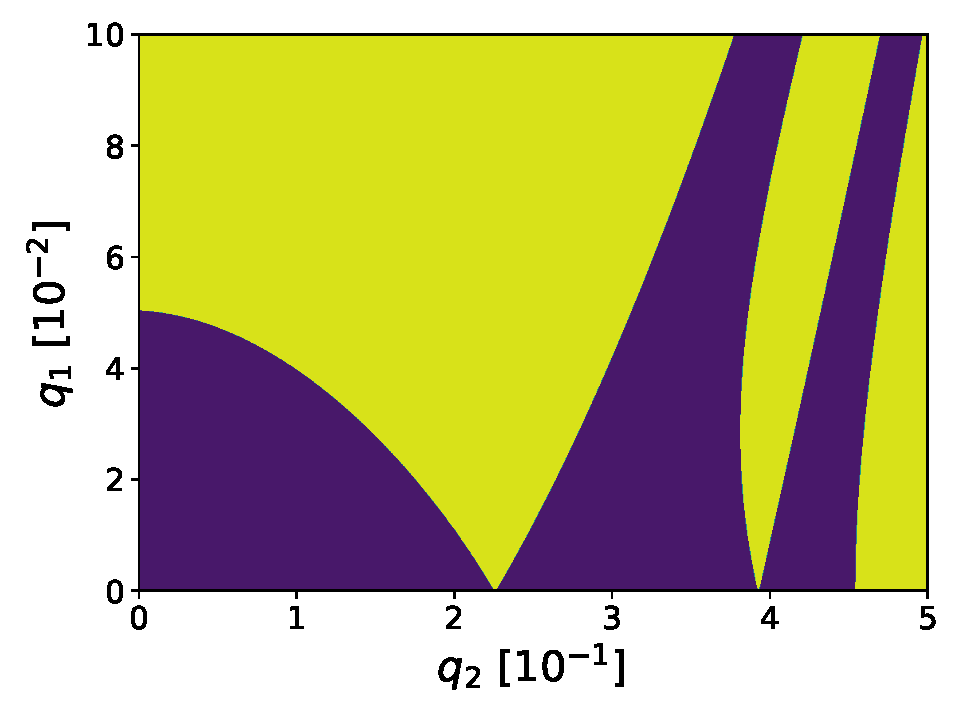
\includegraphics[width=\linewidth]{img/det_q1_0.0-0.1_q2_0.0-0.5_990x990_3.pdf}
  \caption{Determinant}
  \label{fig:det_3}
\end{subfigure}%
\begin{subfigure}{.5\textwidth}
  \centering
  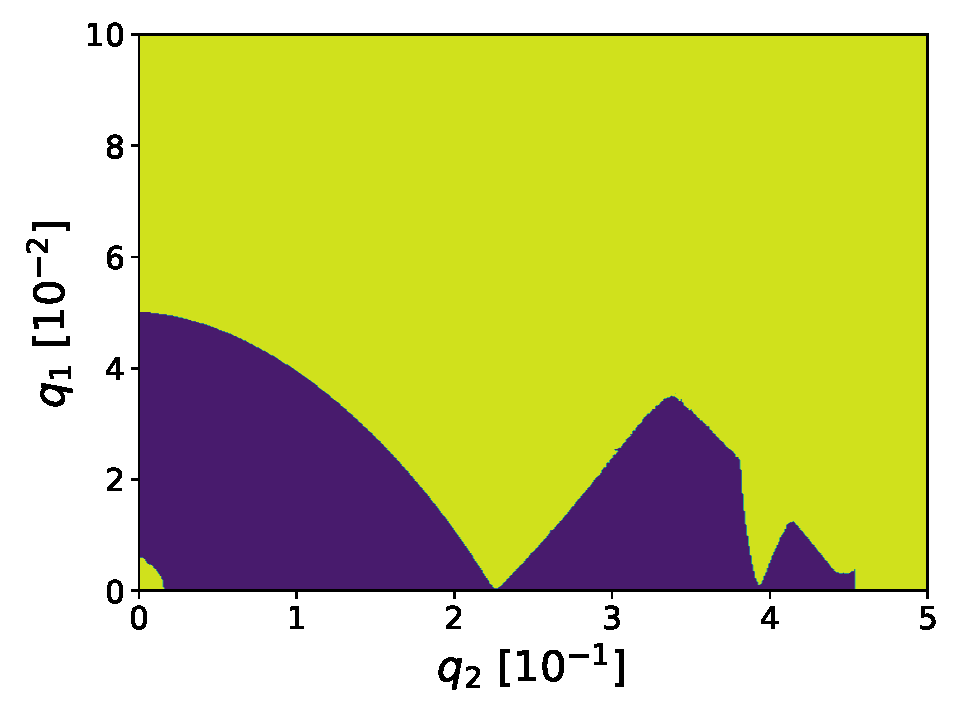
\includegraphics[width=\linewidth]{img/0_ions_1_electrons_q1_0.0-0.1_q2_0.0-0.5_488x488_3.pdf}  
  \caption{Simulation}
  \label{fig:sim_3}
\end{subfigure}
\caption{Stability diagrams for $\nicefrac{\Omega_2}{\Omega_1} = 3$}
\label{fig:stabil-eta=3}
\end{figure}

In the figure \ref{fig:stabil-eta=3} we can see regions of stable\textit{(dark)} and unstable\textit{(light)} solutions to our equation of motion. The picture \ref{fig:det_3} was determined with use of Floquet theory. The adjacent image shows the stability of an electron based on numerical simulation. In contrast with the determinant solution, we can see some evident distinctions. The region around $q_1 \approx q_2 \approx 0$ became unstable. This is no surprise since the weak field simply did not satisfy the stability requirement \eqref{stability condition inequality} for the given initial conditions. More importantly, two whole stability areas have melted away in the field with higher amplitudes. We must not forget that the stability in the figure \ref{fig:det_3} is calculated only along the z-axis. We can investigate this by setting the initial position and velocity in x-y directions to zero. As we can see, the subsequent picture \ref{fig:sim_3_z-direction} already agrees with the determinant solution \ref{fig:det_3}.

\begin{figure}[H]
\begin{subfigure}{.5\textwidth}
  \centering
  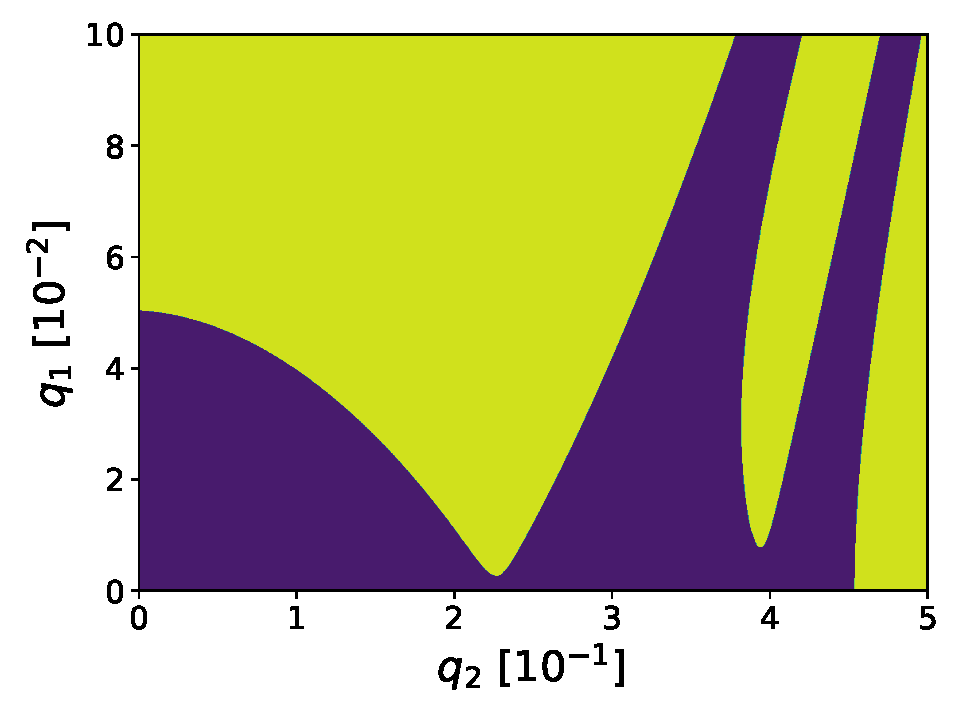
\includegraphics[width=\linewidth]{img/0_ions_1_electrons_q1_0.0-0.1_q2_0.0-0.5_992x992_3.pdf}
  \caption{Simulation in z-direction}
  \label{fig:sim_3_z-direction}
\end{subfigure}%
\begin{subfigure}{.5\textwidth}
  \centering
  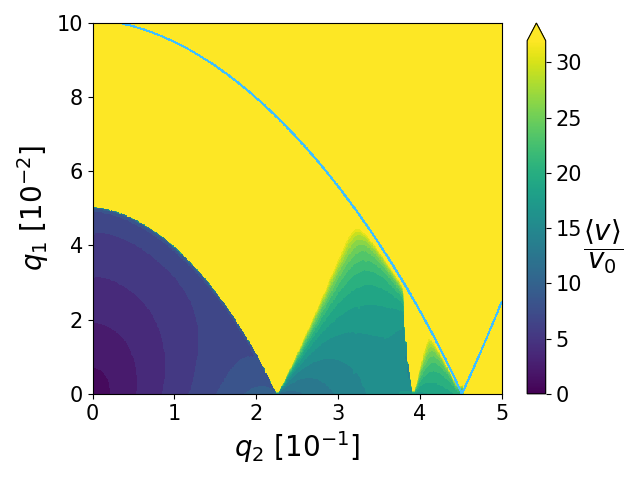
\includegraphics[width=\linewidth]{img/det_q1_0.0-0.1_q2_0.0-0.5_970x970_3_1000.png}  
  \caption{Average velocity simulated in 3D}
  \label{fig:sim_3_x-y_edge}
\end{subfigure}
\caption{Stability diagrams for $\nicefrac{\Omega_2}{\Omega_1} = 3$}
\label{fig:stabil-eta=3 different directions}
\end{figure}

In the next set of pictures \ref{fig:stabil-eta=3_x-y_directions}, we evaluate the stability diagram in x-y directions by setting $\zeta = x$ in \eqref{tilde params} for a determinant solution and setting the z-component of initial position and velocity to zero in the simulation. The red trace in both pictures embodies the edge of stability made with our standard \eqref{stability condition in simulation} stability requirement in simulation. The contour plot in \ref{fig:sim_3_x-direction} was created with the enhanced condition for identifying stable solutions from the standard \eqref{stability condition in simulation} to $\max\limits_{x \in \mathcal{L}}(r) \leq 2 \ \ell_0$, while increasing the total simulation time as well. So the picture \ref{fig:sim_3_x-direction}, among other things, illustrates the non-equivalence of our stability condition in simulation, and the condition we use in Floquet theory, as we have already mentioned in \ref{foot:different stability condition}. 

In the background of \ref{fig:sim_3_x-y_edge} is a contour plot of the average electron velocity $\langle v \rangle$ throughout the whole trajectory\footnote{Average value defined as: $\langle \xi \rangle = \nicefrac{1}{T} \int_{0}^{T} \xi(\tau) \, d\tau,$ where $T$ denotes a total time of simulation.} relative to the initial velocity $v_0$. The color bar to the right indicates the value of this ratio. We create all the other figures similar to \ref{fig:sim_3_x-y_edge} in the same way. These diagrams can help us find stable trap parameters while keeping electron temperature as low as possible, which is our ultimate goal. The light blue line in \ref{fig:sim_3_x-y_edge} represents the stability edge taken from \ref{fig:stabil-eta=3_x-y_directions}, delivering a crucial message about the difference between the two stability diagrams in \ref{fig:stabil-eta=3}. We see that the discrepancy between determinant and simulated stability diagrams is settled by the obvious necessity to combine determinant solutions in both x and z directions. This can be easily fixed with the cost of doubling the computation time for a determinant solution. Nonetheless, from now on, we will focus on simulated results, keeping the determinant diagrams in the z-direction for comparison. Moreover, we can use these pictures \ref{fig:stabil-eta=3_x-y_directions} as a sanity check. By matching them with the results from \cite{leefer2017investigation} \textit{(where the stability of the ideal quadrupole trap along the x-direction was studied)}, we see that we have reproduced the same\footnote{Note that we are using different condition to identify stable solutions.} results $\rightarrow$ proving the validity of our code, at least to some extent.
\begin{figure}[H]
\begin{subfigure}{.5\textwidth}
  \centering
  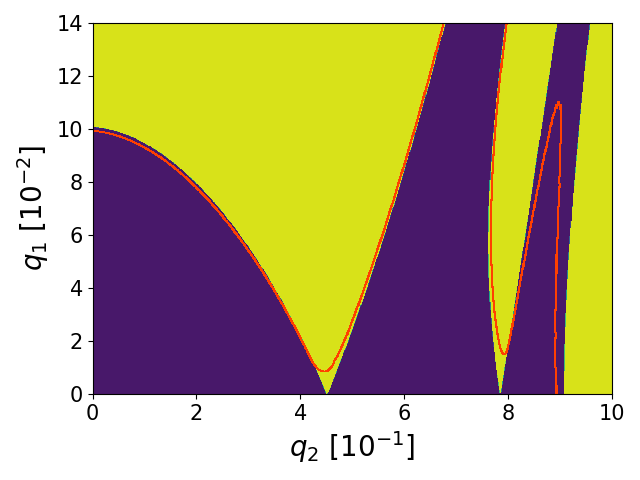
\includegraphics[width=\linewidth]{img/0_ions_1_electrons_q1_0.0-0.14_q2_0.0-1.0_992x984_3_edge.png}%det_q1_0.0-0.14_q2_0.0-1.0_960x960_3.pdf not sure which one to use
  \caption{Determinant in x-direction}
  \label{fig:det_3_x-direction}
\end{subfigure}%
\begin{subfigure}{.5\textwidth}
  \centering
  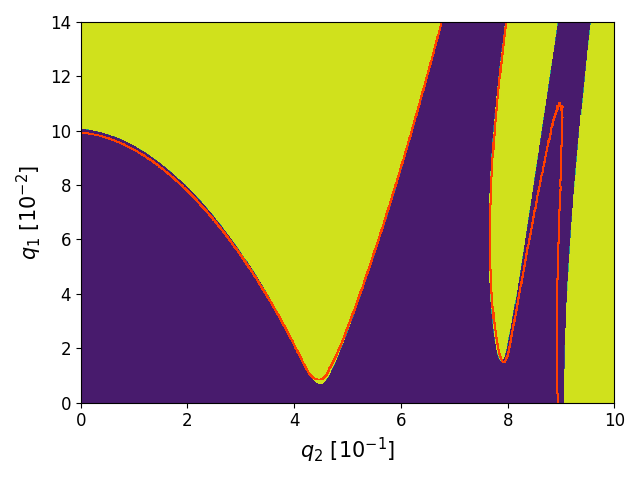
\includegraphics[width=\linewidth]{img/0_ions_1_electrons_q1_0.0-0.14_q2_0.0-1.0_992x984_3_edge_sim.png}  
  \caption{Simulation in x-y plane}
  \label{fig:sim_3_x-direction}
\end{subfigure}
\caption{Stability diagrams for $\nicefrac{\Omega_2}{\Omega_1} = 3$ in x-y plane}
\label{fig:stabil-eta=3_x-y_directions}
\end{figure} 
The image \ref{fig:velocityedge-eta=3} again combines two pictures. Here\textit{(and in all other pictures as well)} the pink curve construes the stable simulated regions, in this case, taken from \ref{fig:sim_3}. 
\begin{figure}[H]
	\centering
	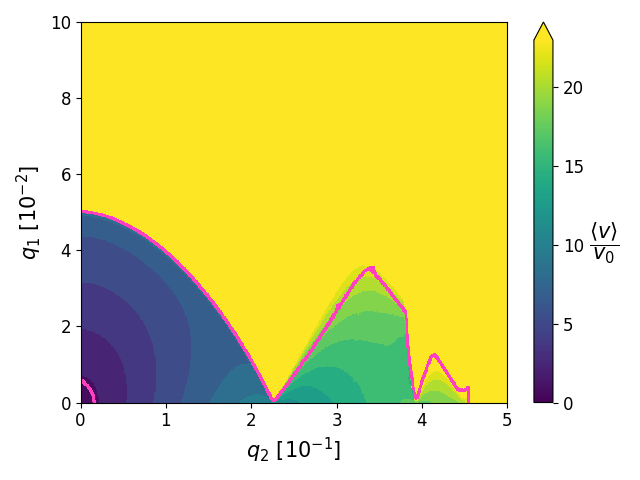
\includegraphics[width=\linewidth]{img/0_ions_1_electrons_q1_0.0-0.1_q2_0.0-0.5_488x488_3_1000.png}
	\caption{Average electron velocity for $\nicefrac{\Omega_2}{\Omega_1} = 3$}
	\label{fig:velocityedge-eta=3}
\end{figure}

Moving to larger frequency ratio $\rightarrow \nicefrac{\Omega_2}{\Omega_1} = 13$ we can start to notice some patterns. There emerges one stable triangle with many tongues of instability. With an increasing ratio $\nicefrac{\Omega_2}{\Omega_1}$ we can see a gain in the number of these tongues, but their width promptly shrinks as well. We can expect that by further increasing the frequency ratio, the unstable tongues will be realistically affecting only the regions near the edge of stability, leaving the regions further inside a stable triangle safe to work with.

\begin{figure}[H]
\begin{subfigure}{.5\textwidth}
  \centering
  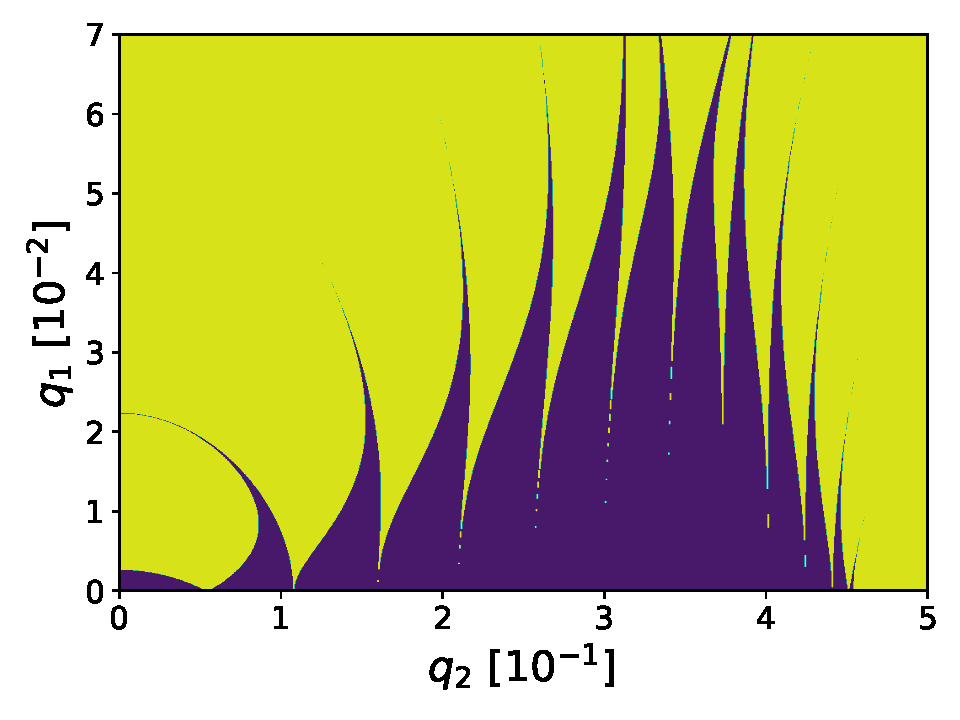
\includegraphics[width=\linewidth]{img/det_q1_0.0-0.07_q2_0.0-0.5_960x960_13.pdf}
  \caption{Determinant}
  \label{fig:det_13}
\end{subfigure}%
\begin{subfigure}{.5\textwidth}
  \centering
  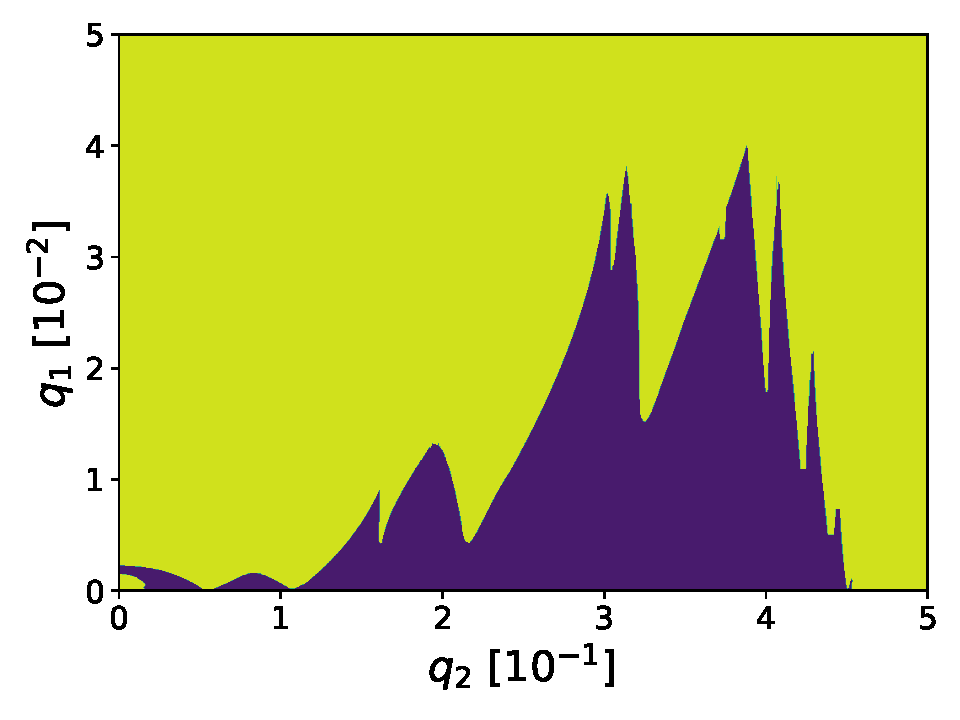
\includegraphics[width=\linewidth]{img/0_ions_1_electrons_q1_0.0-0.05_q2_0.0-0.5_960x960_13.pdf}  
  \caption{Simulation}
  \label{fig:sim_13}
\end{subfigure}
\caption{Stability diagrams for $\nicefrac{\Omega_2}{\Omega_1} = 13$}
\label{fig:velocityedge-eta=13}
\end{figure}

\begin{figure}[H]
	\centering
	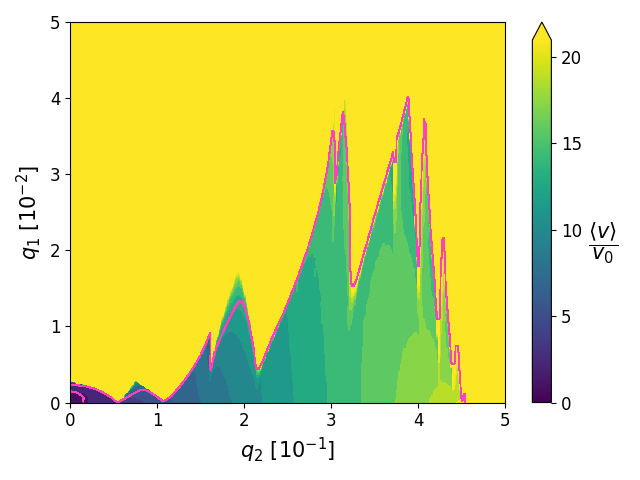
\includegraphics[width=\linewidth]{img/0_ions_1_electrons_q1_0.0-0.05_q2_0.0-0.5_960x960_13_1000.png}
	\caption{Average electron velocity for $\nicefrac{\Omega_2}{\Omega_1} = 13$}
	\label{fig:stabil-eta=13}
\end{figure}

Continuing to the frequency ratio compatible for trapping electrons and Ca+ ions $\rightarrow \nicefrac{\Omega_2}{\Omega_1} = 833$

\begin{figure}[H]
\begin{subfigure}{.5\textwidth}
  \centering
  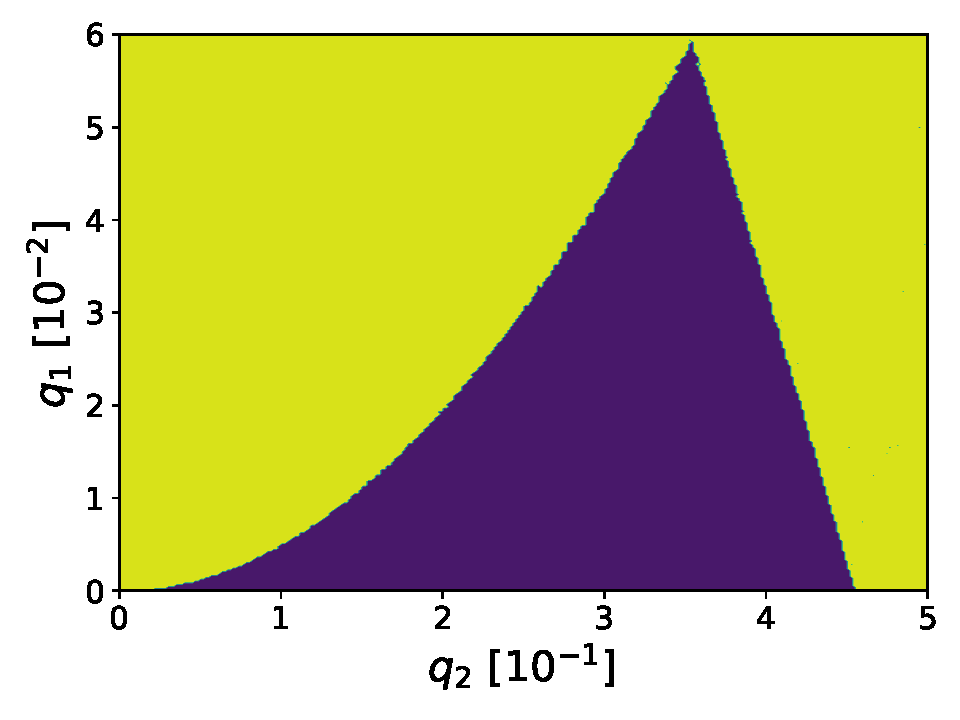
\includegraphics[width=\linewidth]{img/det_q1_0.0-0.06_q2_0.0-0.5_300x300_833.pdf}
  \caption{Determinant}
  \label{fig:det_833}
\end{subfigure}%
\begin{subfigure}{.5\textwidth}
  \centering
  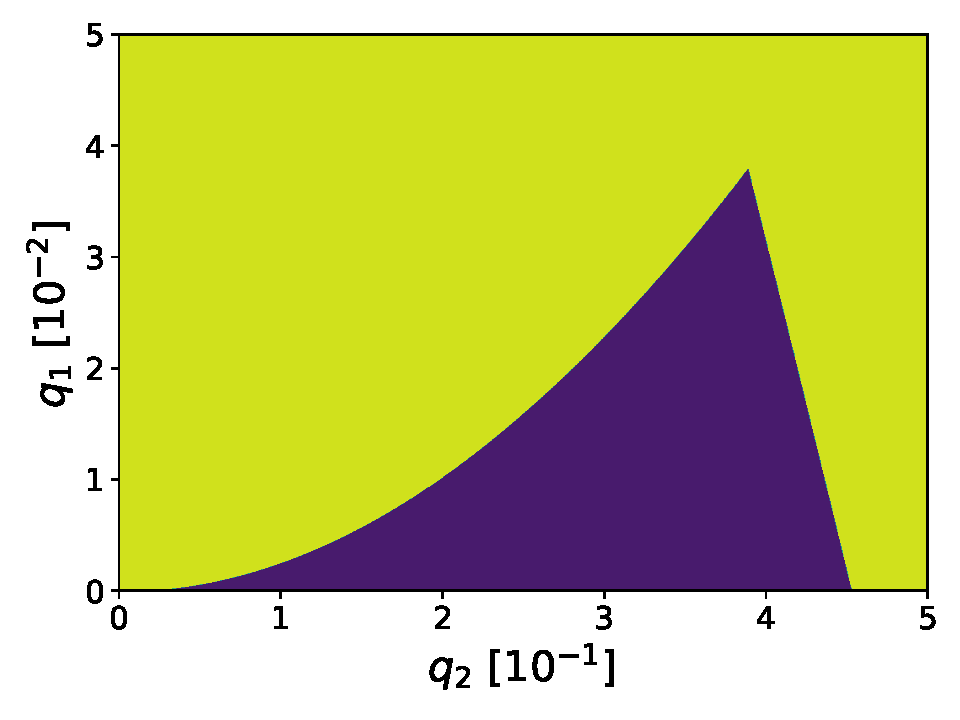
\includegraphics[width=\linewidth]{img/0_ions_1_electrons_q1_0.0-0.05_q2_0.0-0.5_960x960_833.pdf}  
  \caption{Simulation}
  \label{fig:sim_833}
\end{subfigure}
\caption{Stability diagrams for $\nicefrac{\Omega_2}{\Omega_1} = 833$}
\label{fig:stabil-eta=833}
\end{figure}

At this point, the unstable tongues became so dense and narrow that we practically could not see them in stability diagrams \ref{fig:stabil-eta=833}. The closeup on the stability edge \ref{fig:stabil-edge-eta=833} was evaluated after a thousand secular oscillations, and the tongues vanished virtually instantly. The stability triangle will continue to shrink with an increasing frequency ratio. However, the character of this region will stay the same. Therefore, based on the results for $\nicefrac{\Omega_2}{\Omega_1} = 833$, we can even make a rough prediction of stability for different frequency ratios in this range. 

\begin{figure}[H]
	\centering
	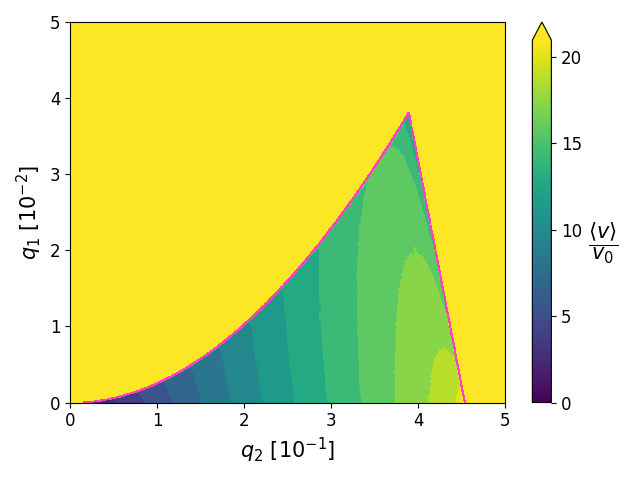
\includegraphics[width=\linewidth]{img/0_ions_1_electrons_q1_0.0-0.05_q2_0.0-0.5_960x960_833_1000.png}
	\caption{Average electron velocity for $\nicefrac{\Omega_2}{\Omega_1} = 833$}
	\label{fig:vel-eta=833}
\end{figure}

\begin{figure}[H]
\begin{subfigure}{.5\textwidth}
  \centering
  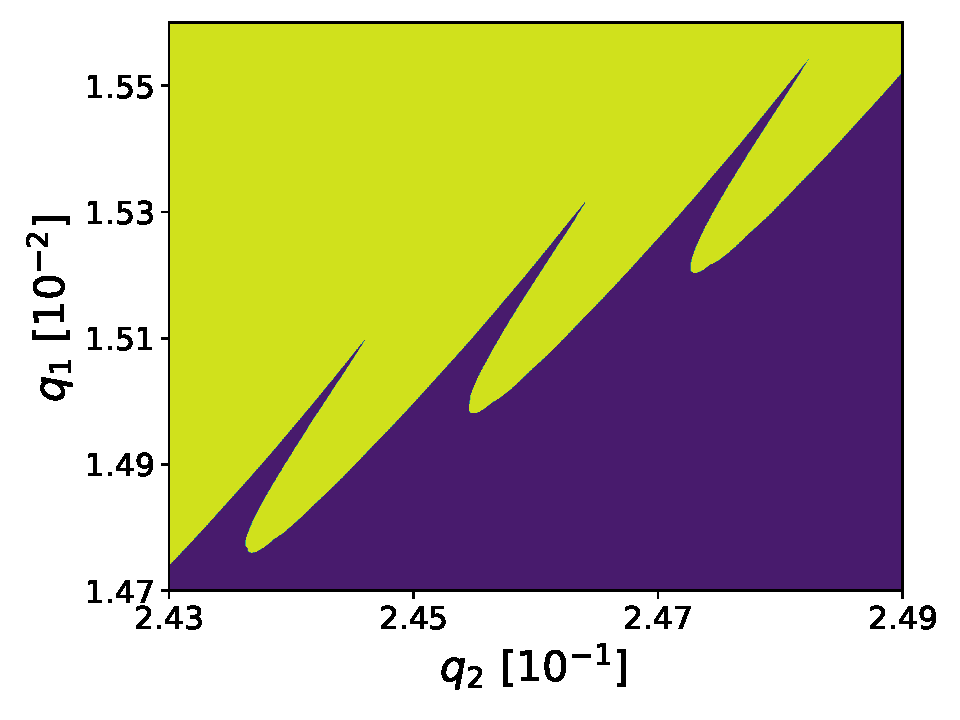
\includegraphics[width=\linewidth]{img/0_ions_1_electrons_q1_0.0147-0.0156_q2_0.243-0.249_960x960_833.pdf}
  %\caption{Determinant}
  \label{fig:sim-edge_833}
\end{subfigure}%
\begin{subfigure}{.5\textwidth}
  \centering
  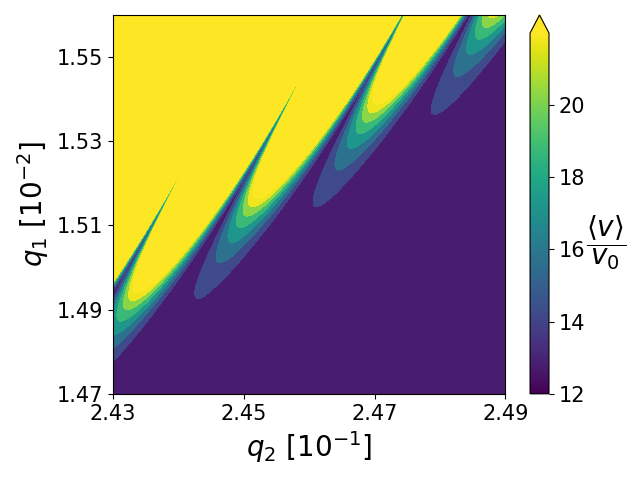
\includegraphics[width=\linewidth]{img/0_ions_1_electrons_q1_0.0147-0.0156_q2_0.243-0.249_220x220_833.png}  
  %\caption{Simulation}
  \label{fig:sim-edge-vel_833}
\end{subfigure}
\caption{Simulated edge of stability for $\nicefrac{\Omega_2}{\Omega_1} = 833$}
\label{fig:stabil-edge-eta=833}
\end{figure}

The essential information comes from the figure \ref{fig:vel-eta=833}. We can see that the electrons' average velocity drops in the fields with a higher $q_1$ parameter. However, there arises an even more reliable tendency of the electrons slowing down in the direction of the weaker fields, furnishing us with a method to reach lower electron velocities. Imagine we have already assembled a CC and managed to trap an electron inside it. Assuming the electron can cool itself by interactions with ions, we can follow by gradual change of trapping parameters aiming towards the weak field region, effectively lowering the electrons' average velocity. This means that we have found the recipe for reaching low temperatures of electrons in two frequency Paul trap. Such a process will be simulated in the future.

It is worth pointing out that the computation time of the determinant stability diagram already exceeds that of simulated for a frequency ratio this big. However, we apply a built-in NumPy\footnote{NumPy is widely used, open source, numerical python library: \href{https://numpy.org}{https://numpy.org/}} function for computing determinants using LU decomposition \cite{teukolsky1992numerical} with time complexity $\mathcal{O}(n^3)$, not utilizing the fact that our matrices are sparse. Moreover, we are interested only in the sign of a determinant, which also supports a capacity for efficiency improvement. But since the determinant solutions are not essential to us, we do not investigate such further advancements in this thesis.

\begin{figure}[H]
	\centering
	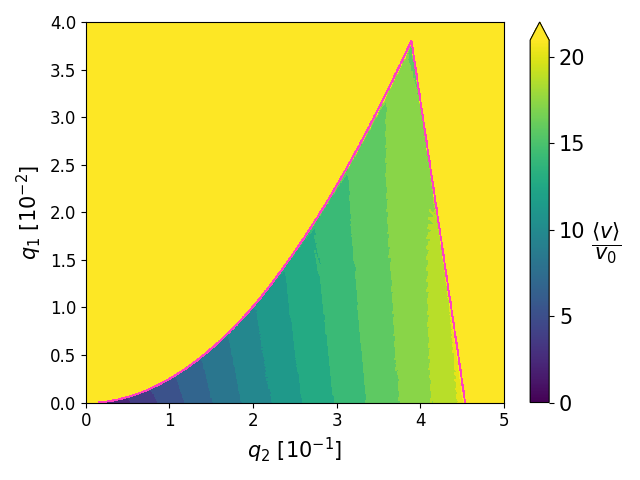
\includegraphics[width=\linewidth]{img/0_ions_1_electrons_q1_0.0-0.04_q2_0.0-0.5_960x960_1207_1000.png}
	\caption{Average electron velocity for $\nicefrac{\Omega_2}{\Omega_1} = 1207$}
	\label{fig:vel-eta=1207}
\end{figure}

We produced one more diagram showing stability and average electron velocity for the different ratio of driving frequencies. As predicted, solutions with lower frequency $\omega_1$ are less stable but show similar qualities as \ref{fig:vel-eta=833}.

\section{Creating a Coulomb crystal}
As we have already mentioned, we assemble a CC by solving the equation of motion for each ion in an effective potential with damping and mutual Coulombic interaction. Meaning that the equation of motion for the i-th ion takes the form:
\begin{equation}
	\label{eomCC}
	M_{ion}\vb{\ddot{R}}_i = \sum\limits_{\substack{j=1 \\ j\neq i}}^{N} \frac{Q^2}{4 \pi \varepsilon_0} \frac{\vb{R_i} \minus \vb{R_j}}{|\vb{R_i} \minus \vb{R_j}|^3} \minus  \frac{M_{el}^2 \Omega_2^2}{8 M_{ion}} \left( \left(\nicefrac{\Omega_2}{\Omega_1}\right)^2 q_1^2 + q_2^2 \right) \begin{bmatrix}
		x_i \\
		y_i \\
		4z_i
	\end{bmatrix} \minus \beta \vb{\dot{R}}_i,
\end{equation}
where here, the vector $\vb{R}$ denotes a position of a concrete ion. For these simulations, we have made a classic choice of implementing Verlet integration with the constant time-step. We have tried using a custom adaptive time-step, looking at relative positions and velocities of particles. However, this approach turned out to be less efficient. Nevertheless, such a time-step will be preferred once we start investigating the stability while allowing the possibility of recombination.

\begin{figure}[H]
\begin{subfigure}{.5\textwidth}
  \centering
  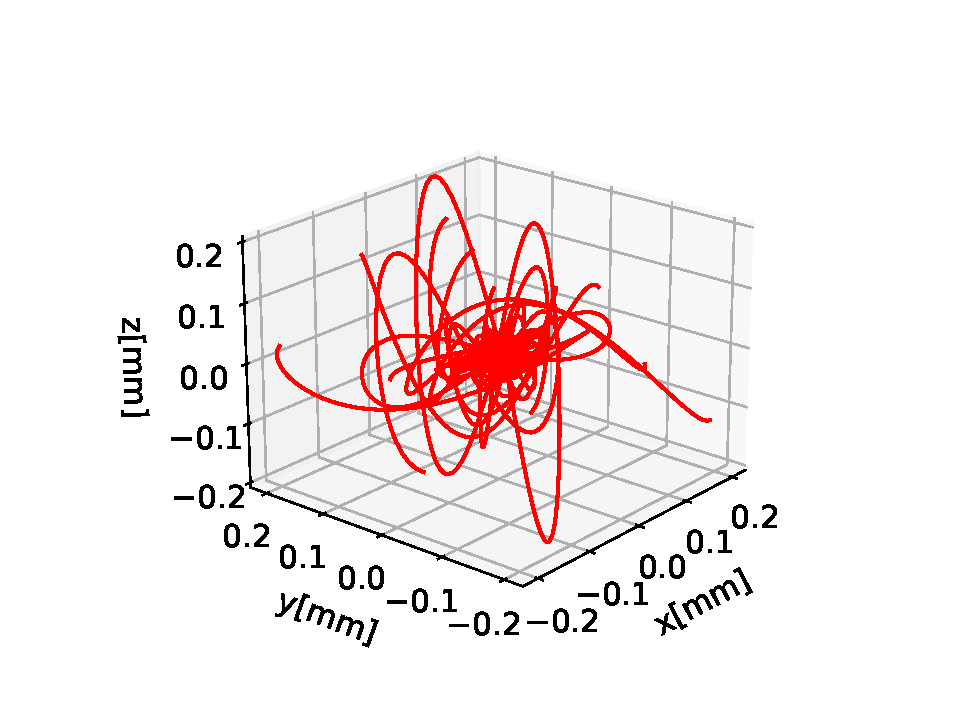
\includegraphics[width=\linewidth]{img/CC_10.pdf}
  \caption{Simulating multiple ions in effective potential with damping}
\end{subfigure}%
\begin{subfigure}{.5\textwidth}
  \centering
  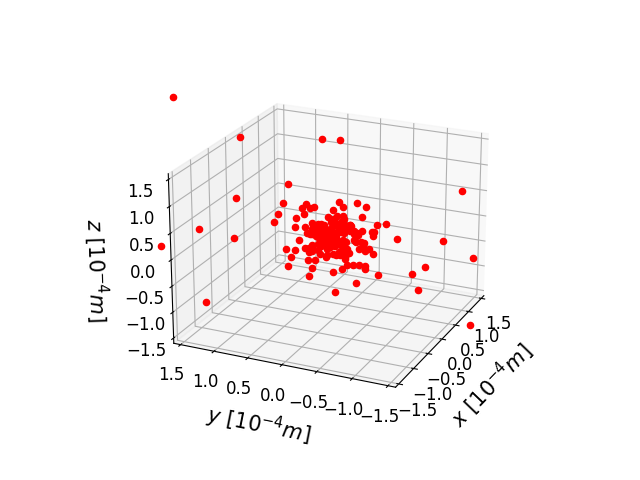
\includegraphics[width=\linewidth]{img/CC_200.png}  
  \caption{Process of assembling a CC (200 ions)}
\end{subfigure}
\caption{Creating CC $\nicefrac{\Omega_2}{\Omega_1} = 1207$}
\label{fig:CC-eta=1207}
\end{figure}

\section{Stability of electron in Coulomb crystal}
The ions stand practically still in the time scales of $\sim 20$ secular electron oscillations. Therefore, while computing stability diagrams in the presence of CCs, we freeze ions in place, rapidly improving computational time. We have performed such simulations with up to 200 ions, solving the equation for a i-th electron in the variable $\tau = \nicefrac{t\Omega_2}{2}$:
\begin{multline}
	\label{eq of motion for electrons in CC}
	\vb{\ddot{r}}_i = \frac{Q^2}{\pi M_{el} \varepsilon_0 \Omega_2^2} \left( \sum\limits_{\substack{j=1 \\ j \neq i}}^{N_j} \frac{\vb{r}_i \minus \vb{r}_j}{|\vb{r}_i \minus \vb{r}_j|^3} \minus \sum\limits_{\substack{k=1}}^{N_k} \frac{\vb{r}_i \minus \vb{R}_k}{|\vb{r}_i \minus \vb{R}_k|^3} \right) \\ \minus \big( a \minus 2q_1 \cos\left(2\tau\nicefrac{\Omega_1}{\Omega_2}\right) \minus 2q_2\cos\left(2\tau\right) \big) \begin{bmatrix}
		x\\
		y\\
		-2z
	\end{bmatrix},
\end{multline}
where $\vb{r}_j$ denotes a position of j-th electron, and $\vb{R}_k$ is the constant position of k-th ion. $N_j$ and $N_k$ are the total numbers of electrons and ions respectively. We have simulated stability diagrams by solving equation \eqref{eq of motion for electrons in CC} for multiple CCs, and frequency ratios $\nicefrac{\Omega_2}{\Omega_1} = 833$ and $\nicefrac{\Omega_2}{\Omega_1} = 1207$. However, we did not observe any noticeable differences in contrast to results obtained without the presence of CCs. Nevertheless, some instabilities may arise on longer time scales, which we did not manage to inspect in detail in this thesis because of exhaustive computational durations of these simulations. However, such possible instabilities will be investigated in the future. 

\section{Future}
Our future concerns will begin by continuing the study of electrons' stability in the presence of CC on longer time scales and adding the option of electron cooling via interactions with ions. Another leap will be reproducing the results of this thesis for the real planar geometry of the trap used in our experiment. The potential of such a trap can be formulated in integral form utilizing Bessel functions, making our simulations much more computationally expensive. We need to derive the equation of motion and identify parameters analogous to $a$, $q_1$, and $q_2$, which we had for the ideal quadrupole trap. After that, we can use our exiting program to study the stability and average particle velocity in dependence on such parameters exactly as we did in this thesis. 

\chapter{Future work}
\label{chap:refs}

\chapwithtoc{Conclusion}

In this thesis, we have proposed a design of an experiment in which we might be able to assemble a stable Coulomb crystal with electrons trapped inside. Hopefully, we will cool these electrons to the point when they form a Fermi gas. If successful, such an experiment would advance current options in the research of quantum systems.

We have presented a comprehensive overview of the current state of knowledge regarding the trapping of charged particles solely by an electric field. We have focused on using the ideal Paul trap. We exhibit the supremacy of trapping with two frequencies instead of one for the confinement of two species with widely different charge-to-mass ratios. By reproducing results for trapping in one direction from reviewed scientific articles, we have confirmed the validity of our simulations. After that, we continued producing novel results by studying the stability of electrons in all spatial directions.

We have developed a computer program to simulate charged particles' motion inside the Paul trap. We have used this program to study the stability of particles in dependence on the trap settings, identifying whole areas of stable operating conditions. In the same way, we have evaluated an average electron velocity throughout the trajectory. Based on these results, we propose a technique to achieve lower electron temperatures. To model such a process, we must add a feature to our program representing electrons' possibility to cool themselves by interaction with ions. 

\xxx{This and this was performed and this and this will be extended in the future to assist in determination of optimal experimental conditions for studies of low energy ion-electron interactions. Namely this and this have to done\dots}


\ifEN
\chapwithtoc{Bibliography}
\else
\chapwithtoc{Seznam použité literatury}
\fi

\printbibliography[heading=none]

\appendix
\chapter{Using software}

This appendix intends to explain to the reader how to use the python script. The program starts by running the \verb|main.py| file. In this file there are definition of function which uses more complex functionalities from the other modules. When running the \verb|main.py| one should uncomment all the lines he/she want to be executed (see \ref{lst:main}).

\xxx{This is an example code.}

\begin{Verbatim}
def StepVerlet(ODESystem, rv, t, dt, aCoulomb, mass, charge, trapParams):

    r, v = rv
    v, a = ODESystem(rv, t, aCoulomb, mass, charge, trapParams)
    
    r1 = r + v * dt + 0.5 * a * dt**2
    
    a1 = ODESystem(np.array([r1, v]), t, aCoulomb, mass, charge, trapParams)[1]    
    
    v1 = v + 0.5 * (a + a1) * dt
    t1 = t + dt
    
    rv1 = np.array([r1, v1])
    
    return rv1, t1   
\end{Verbatim}


\begin{listing}
\begin{lstlisting}
if __name__ == '__main__':
    
    prayForItToWork()
	    
\end{lstlisting}
\caption{Main program.}
\label{lst:main}
\end{listing}


% if your attachments are complicated, describe them in a separate appendix
%\include{attachments}

\openright
\end{document}
